% 本模板根据中国科学院大学本科生公共必修课程《基础物理实验》Word模板格式编写
% 本模板由Shing-Ho Lin和Jun-Xiong Ji于2022年9月共同完成, 旨在方便LaTeX原教旨主义者和被Word迫害者写实验报告, 避免Word文档因插入过多图与公式造成卡顿. 
% 如有任何问题, 请联系: linchenghao21@mails.ucas.ac.cn
% This is the LaTeX template for experiment report of Experimental Physics courses, based on its provided Word template. 
% This template is completed by the joint collabration of Shing-Ho Lin and Junxiong Ji in September 2022. 
% Adding numerous pictures and equations leads to unsatisfying experience in Word. Therefore LaTeX is better. 
% Feel free to contact us via: linchenghao21@mails.ucas.ac.cn

\documentclass[11pt]{article}

\usepackage[a4paper]{geometry}
\geometry{left=2.0cm,right=2.0cm,top=2.5cm,bottom=2.5cm}

\usepackage{ctex} % 支持中文的LaTeX宏包
\usepackage{amsmath,amsfonts,graphicx,subfigure,amssymb,bm,amsthm,mathrsfs,mathtools,breqn} % 数学公式和符号的宏包集合
\usepackage{algorithm,algorithmicx} % 算法和伪代码的宏包
\usepackage[noend]{algpseudocode} % 算法和伪代码的宏包
\usepackage{fancyhdr} % 自定义页眉页脚的宏包
\usepackage[framemethod=TikZ]{mdframed} % 创建带边框的框架的宏包
\usepackage{fontspec} % 字体设置的宏包
\usepackage{adjustbox} % 调整盒子大小的宏包
\usepackage{fontsize} % 设置字体大小的宏包
\usepackage{tikz,xcolor} % 绘制图形和使用颜色的宏包
\usepackage{multicol} % 多栏排版的宏包
\usepackage{multirow} % 表格中合并单元格的宏包
\usepackage{pdfpages} % 插入PDF文件的宏包
\RequirePackage{listings} % 在文档中插入源代码的宏包
\RequirePackage{xcolor} % 定义和使用颜色的宏包
\usepackage{wrapfig} % 文字绕排图片的宏包
\usepackage{bigstrut,multirow,rotating} % 支持在表格中使用特殊命令的宏包
\usepackage{booktabs} % 创建美观的表格的宏包
\usepackage{circuitikz} % 绘制电路图的宏包

\definecolor{dkgreen}{rgb}{0,0.6,0}
\definecolor{gray}{rgb}{0.5,0.5,0.5}
\definecolor{mauve}{rgb}{0.58,0,0.82}
\lstset{
  frame=tb,
  aboveskip=3mm,
  belowskip=3mm,
  showstringspaces=false,
  columns=flexible,
  framerule=1pt,
  rulecolor=\color{gray!35},
  backgroundcolor=\color{gray!5},
  basicstyle={\small\ttfamily},
  numbers=none,
  numberstyle=\tiny\color{gray},
  keywordstyle=\color{blue},
  commentstyle=\color{dkgreen},
  stringstyle=\color{mauve},
  breaklines=true,
  breakatwhitespace=true,
  tabsize=3,
}

% 轻松引用, 可以用\cref{}指令直接引用, 自动加前缀. 
% 例: 图片label为fig:1
% \cref{fig:1} => Figure.1
% \ref{fig:1}  => 1
\usepackage[capitalize]{cleveref}
% \crefname{section}{Sec.}{Secs.}
\Crefname{section}{Section}{Sections}
\Crefname{table}{Table}{Tables}
\crefname{table}{Table.}{Tabs.}

\setmainfont{Palatino Linotype.ttf}
\setCJKmainfont{SimHei.ttf}
\setCJKsansfont{Songti.ttf}
\setCJKmonofont{SimSun.ttf}
\punctstyle{kaiming}
% 偏好的几个字体, 可以根据需要自行加入字体ttf文件并调用

\renewcommand{\emph}[1]{\begin{kaishu}#1\end{kaishu}}

%改这里可以修改实验报告表头的信息
\newcommand{\experiName}{光学基础实验}
\newcommand{\supervisor}{左战春}
\newcommand{\name}{张欣培}
\newcommand{\studentNum}{2022K8009922001}
\newcommand{\class}{01}
\newcommand{\group}{07}
\newcommand{\seat}{}
\newcommand{\dateYear}{2023}
\newcommand{\dateMonth}{9}
\newcommand{\dateDay}{25}
\newcommand{\room}{教705}
\newcommand{\others}{$\square$}
%% 如果是调课、补课, 改为: $\square$\hspace{-1em}$\surd$
%% 否则, 请用: $\square$
%%%%%%%%%%%%%%%%%%%%%%%%%%%

\begin{document}

%若需在页眉部分加入内容, 可以在这里输入
% \pagestyle{fancy}
% \lhead{\kaishu 测试}
% \chead{}
% \rhead{}

\begin{center}
    \LARGE \bf 《\, 基\, 础\, 物\, 理\, 实\, 验\, 》\, 实\, 验\, 报\, 告
\end{center}

\begin{center}
    \noindent \emph{实验名称}\underline{\makebox[25em][c]{\experiName}}
    \emph{指导教师}\underline{\makebox[8em][c]{\supervisor}}\\
    \emph{姓名}\underline{\makebox[6em][c]{\name}} 
    % 如果名字比较长, 可以修改box的长度"6em"
    \emph{学号}\underline{\makebox[10em][c]{\studentNum}}
    \emph{分班分组及座号} \underline{\makebox[5em][c]{\class \ -\ \group \ -\ \seat }\emph{号}} (\emph{例}:\, 1\,-\,04\,-\,5\emph{号})\\
    \emph{实验日期} \underline{\makebox[3em][c]{\dateYear}}\emph{年}
    \underline{\makebox[2em][c]{\dateMonth}}\emph{月}
    \underline{\makebox[2em][c]{\dateDay}}\emph{日}
    \emph{实验地点}\underline{{\makebox[4em][c]\room}}
    \emph{调课/补课} \underline{\makebox[3em][c]{\others\ 是}}
    \emph{成绩评定} \underline{\hspace{5em}}
    {\noindent}
    \rule[8pt]{17cm}{0.2em}
\end{center}

\begin{center}
    \Large \bf 第一部分\qquad 实验内容
\end{center}

\section{实验目的}

\begin{enumerate}
    \item 了解与熟悉激光基本原理
    \item 搭建光路,观测激光传输,扩束
    \item 搭建马赫-曾德干涉仪
    \item 通过检偏器了解光的偏振
    \item 观察夫琅和费衍射和光栅衍射现象。
\end{enumerate}

\section{实验器材}

    \hspace*{2em} 
    氦氖激光器,反射镜,分光棱镜,凹凸透镜组,偏振片(起偏器、检偏器),万用表,分划板,激光防护镜等。

\section{实验原理}
\begin{enumerate}
    \item 激光是单色性好、方向性好,亮度更高的光源,其特性便于光学实验的进行。激光的原理是受激辐射光扩大。氦氖激光器中,Ne是工作物质,He是辅助物质。激光良好地沿直线传播。
    \item 光是电磁波,是横波,能够发生波的干涉。光能够偏振。
    \item 光波穿过小孔/小缝时发生衍射现象。
\end{enumerate}


\section{实验内容}


\begin{enumerate}
    \item 马赫-曾德干涉仪
    \begin{enumerate}
        \item 如图搭建光路。激光要先经过反射镜两次反射后,才能继续使用。要保证光通过各个镜面时都保持在同一水平高度,需要多次使用光圈和尺子确定光的高度。凸透镜与凹透镜的距离12cm是凸透镜焦距15cm减去凹透镜焦距3cm。应从透镜平的一面入射。
              \newline 调整光路准直时,“近调近,远调远”,重复几次后能够较为精准地调整光路准直。
        \item 多次调整光路后,生成干涉条纹。我使用的激光器本身会产生两个椭圆光斑,会对条纹有较小影响。光路准直调整的越精确,条纹越明显。调整光路准直时,用光屏在光路出射处远近移动,保证远近都为同一光斑即为调整良好。这是为了保证两束出射光完全重合。
        
        %下面是图片
        \begin{figure}[H]
            \centering
            \begin{minipage}[t]{0.49\linewidth}
                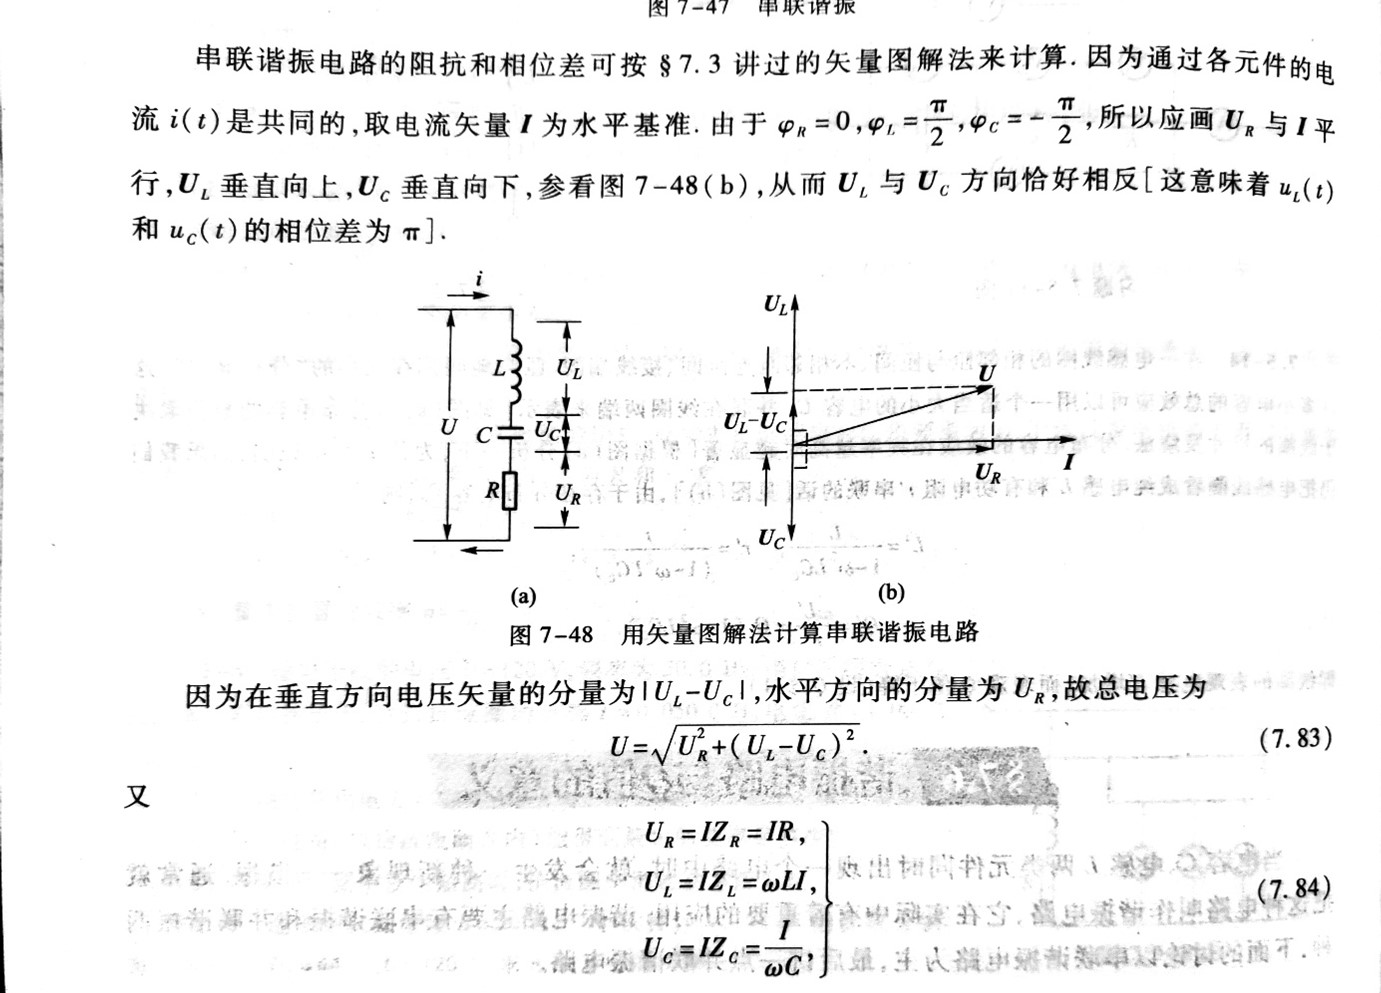
\includegraphics[width=8cm]{Fig/1.jpg}
                \caption{干涉仪光路}
            \end{minipage}
            \begin{minipage}[t]{0.49\linewidth}
                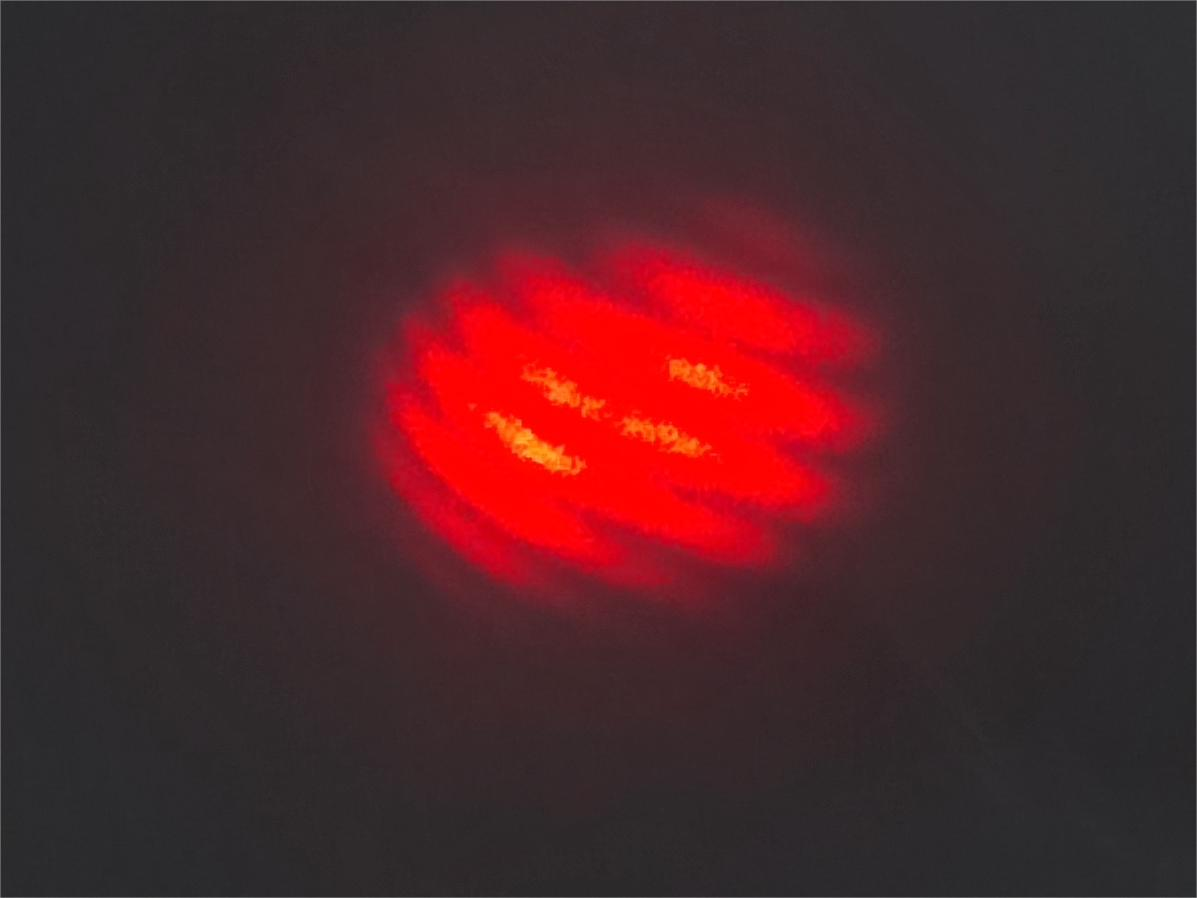
\includegraphics[width=8cm]{Fig/2.jpg}
                \caption{干涉条纹}
            \end{minipage}
            
        \end{figure}

    \end{enumerate}
    \item 夫琅和费衍射和光栅衍射现象
    \begin{enumerate}
        \item 如图搭建光路。在干涉仪的基础上,只保留两个反射镜,加入分划板。图像如下所示。
        
        %下面是图片
        \begin{figure}[H]
            \centering
            \subfigure[]{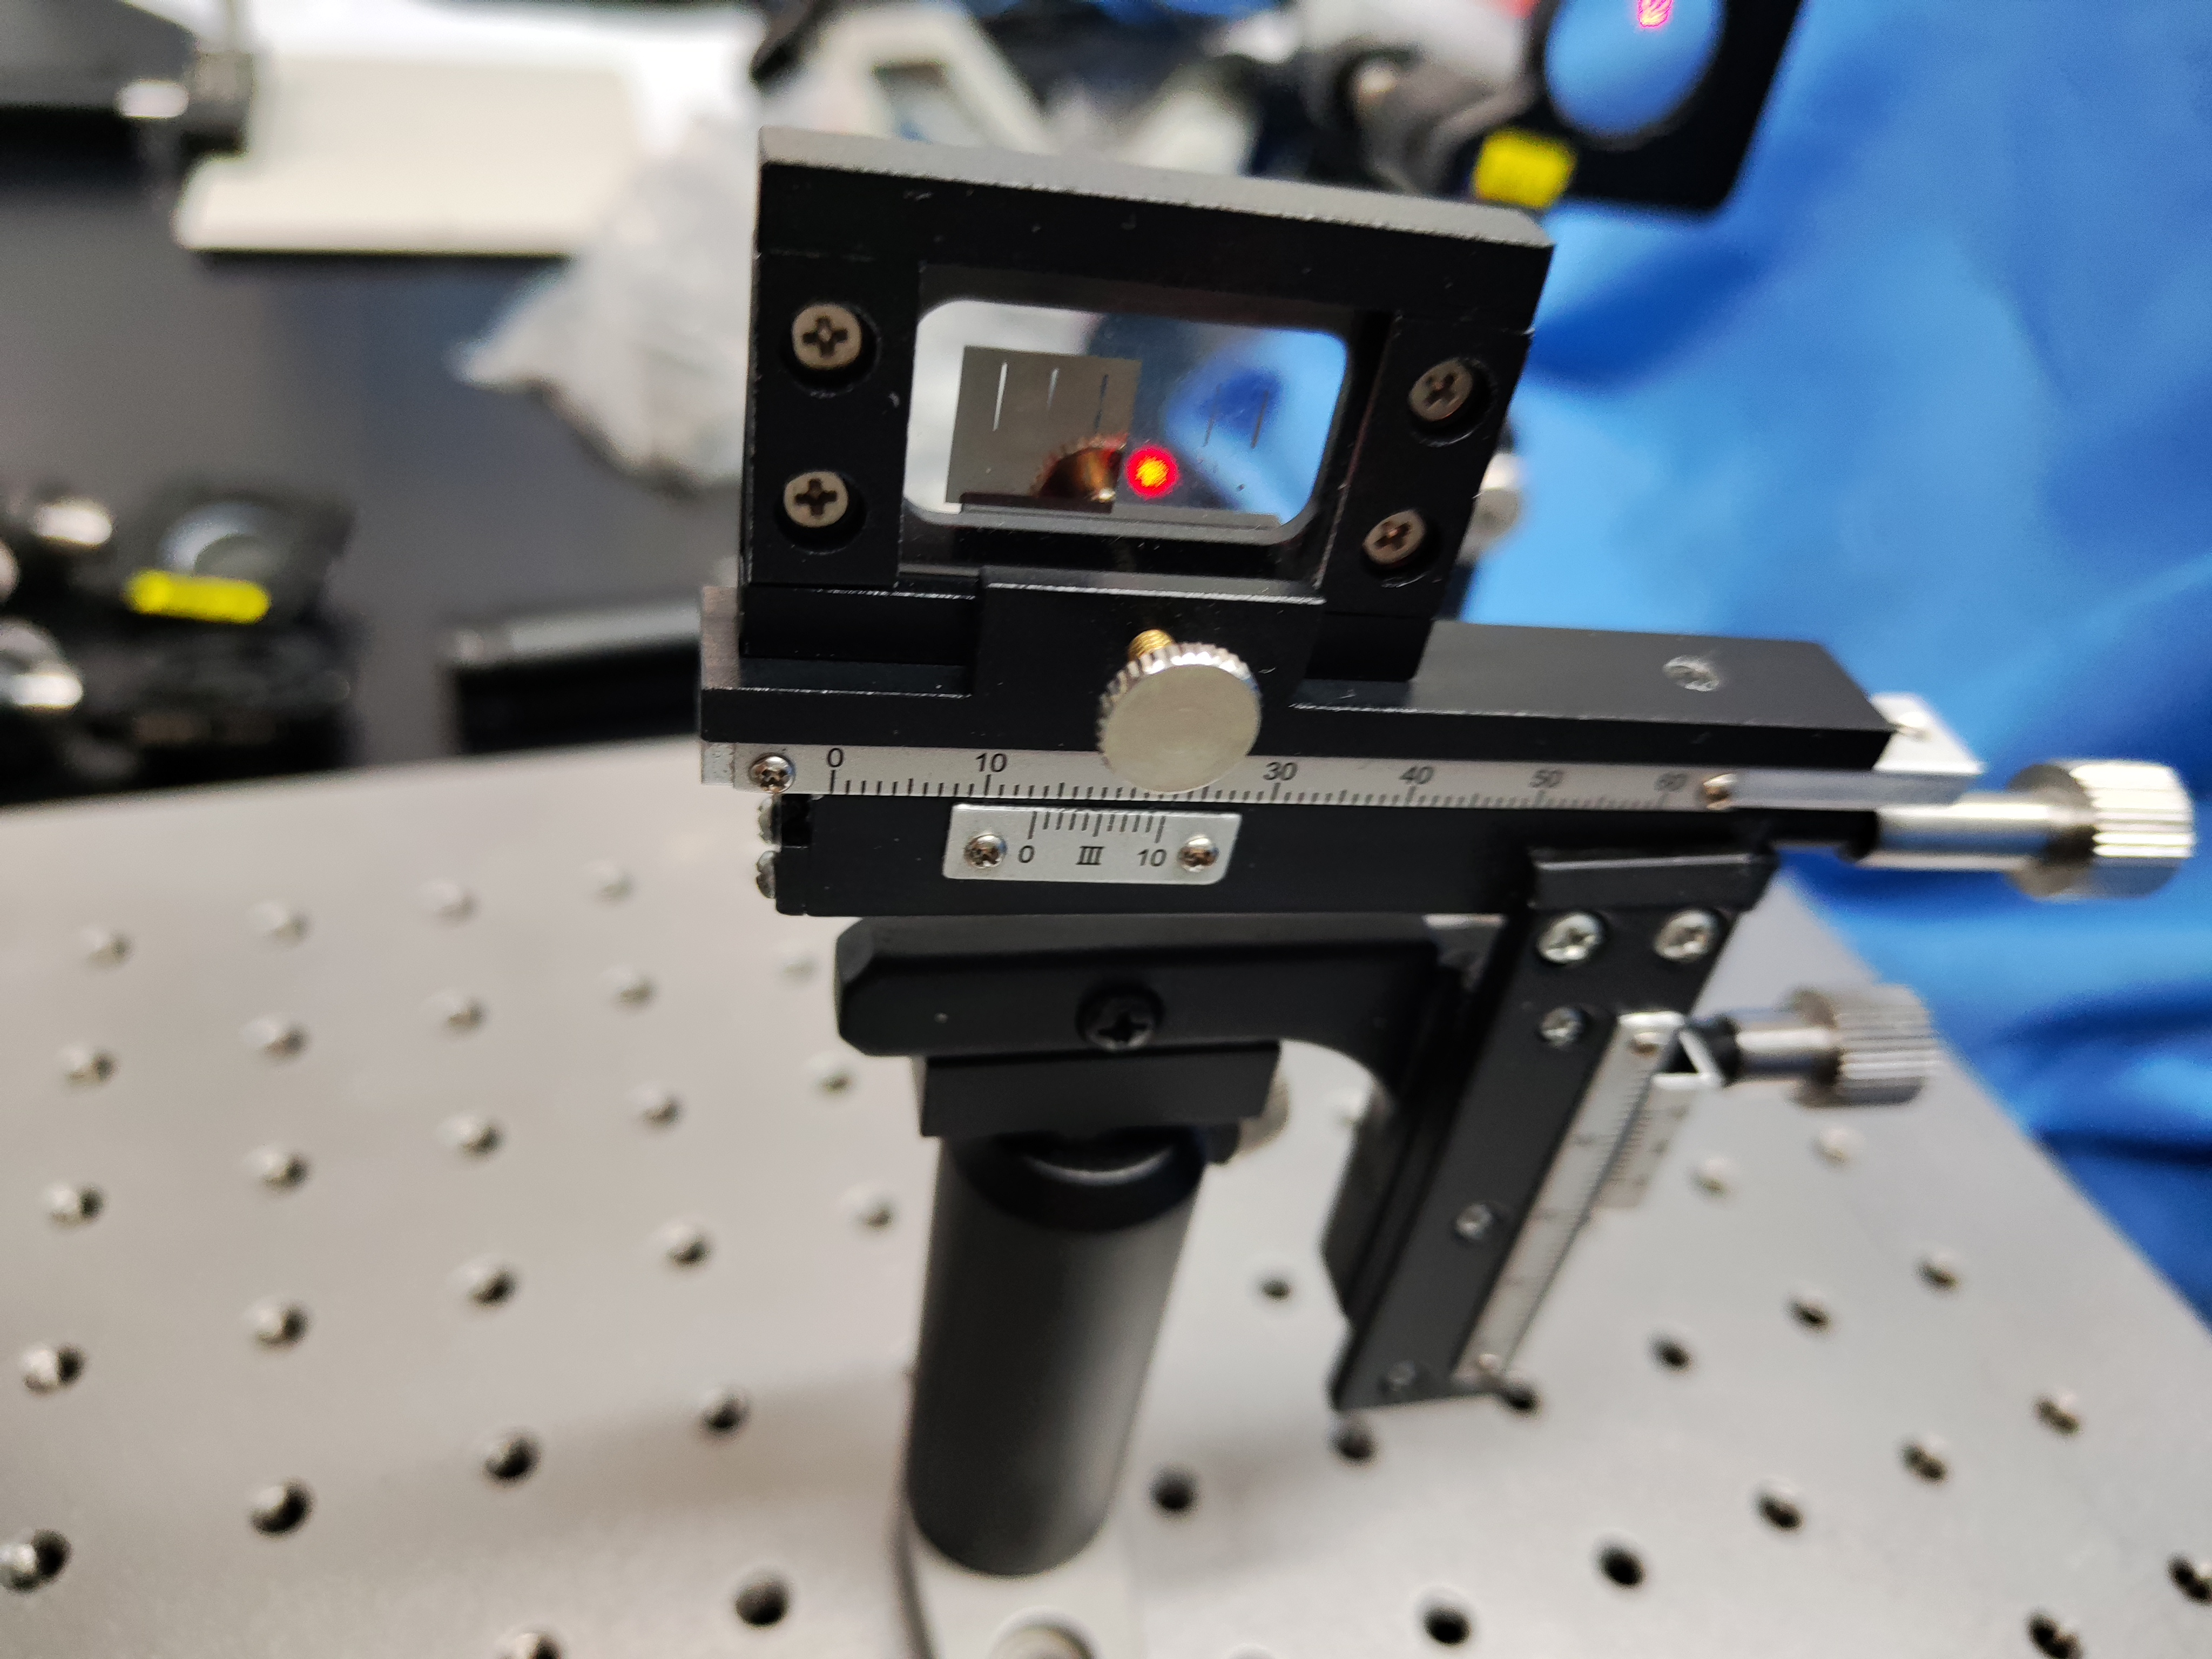
\includegraphics[width=7.5cm]{Fig/3 (1).jpg}}
            \hspace{0.5in}
            \subfigure[]{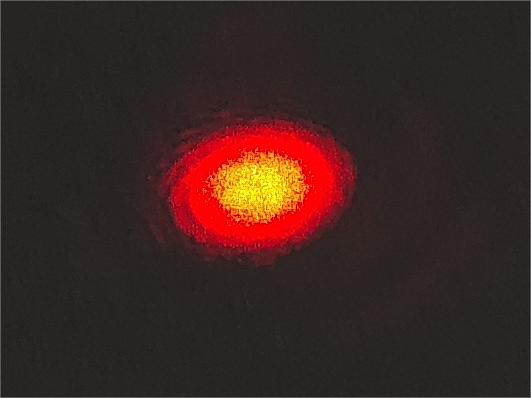
\includegraphics[width=7.5cm]{Fig/3 (2).jpg}}
            \hspace{0.5in}
            \caption{衍射图案}
        \end{figure}
        \begin{figure}[H]
            \centering
            \subfigure[]{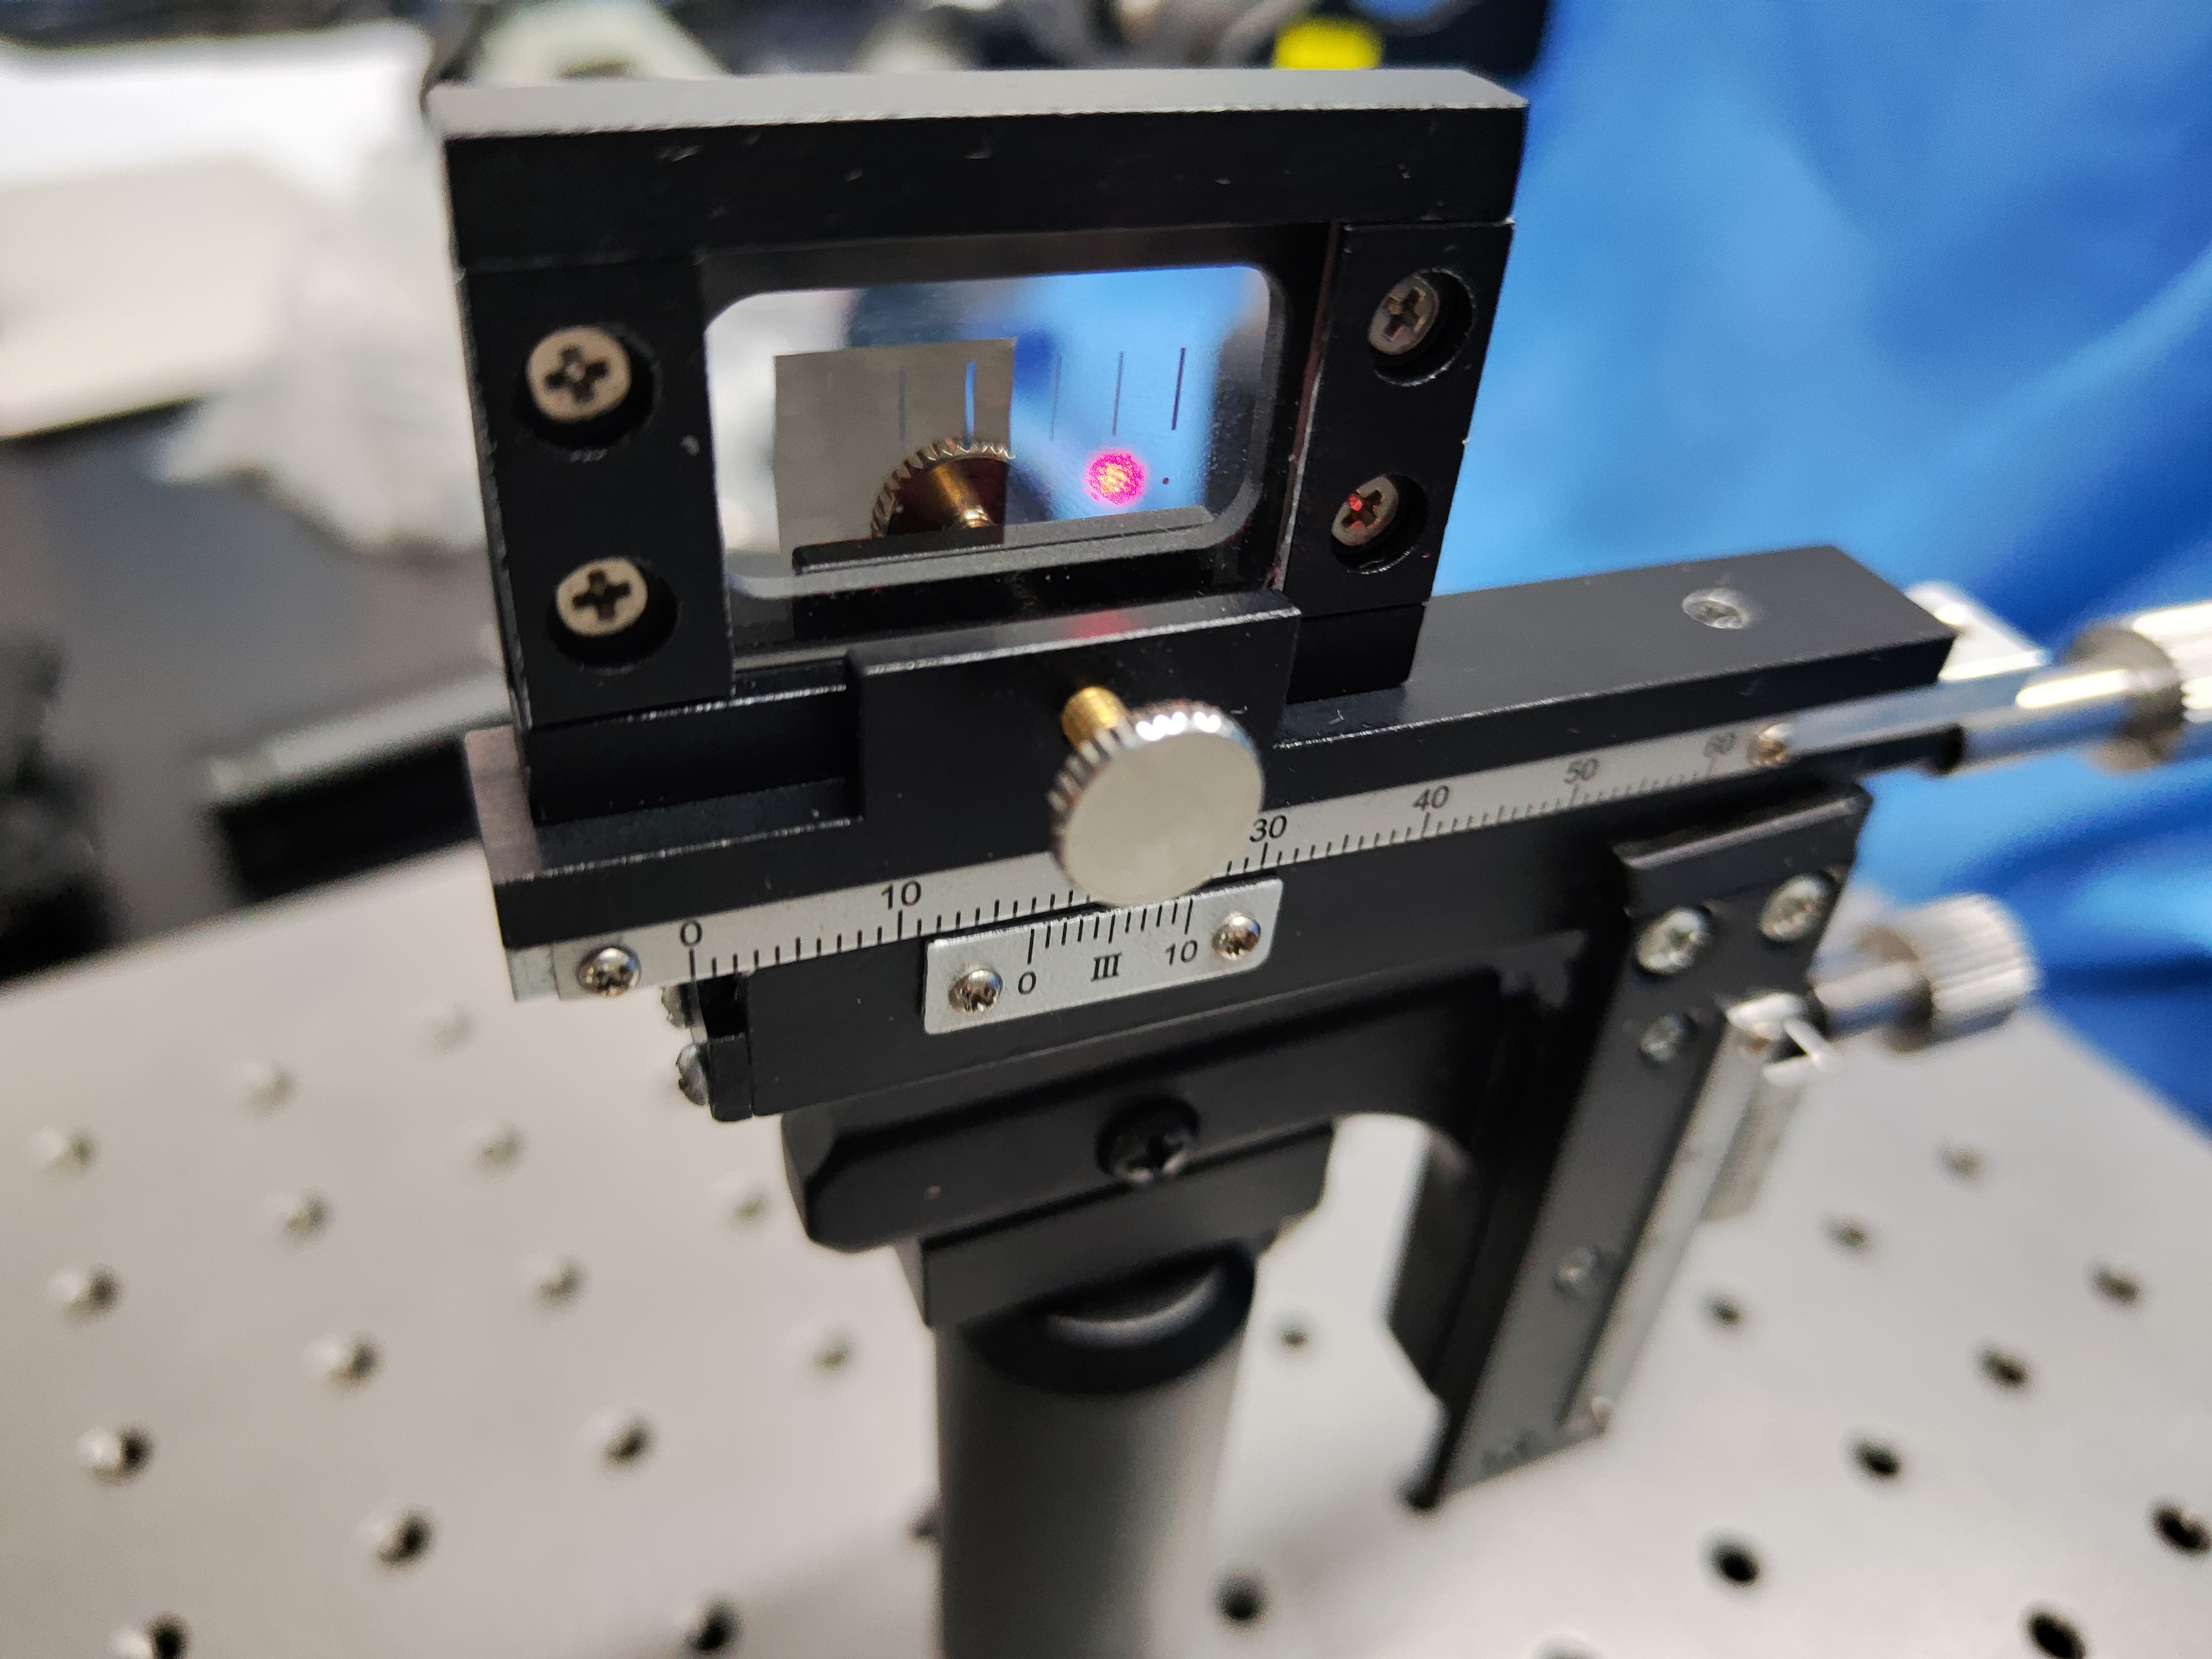
\includegraphics[width=7.5cm]{Fig/3 (3).jpg}}
            \hspace{0.5in}
            \subfigure[]{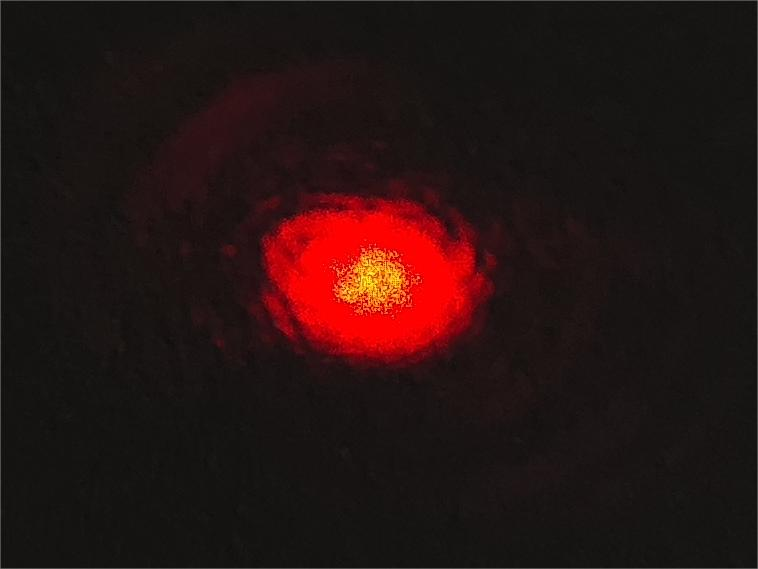
\includegraphics[width=7.5cm]{Fig/3 (4).jpg}}
            \hspace{0.5in}
            \caption{衍射图案}
        \end{figure}
        \begin{figure}[H]
            \centering
            \subfigure[]{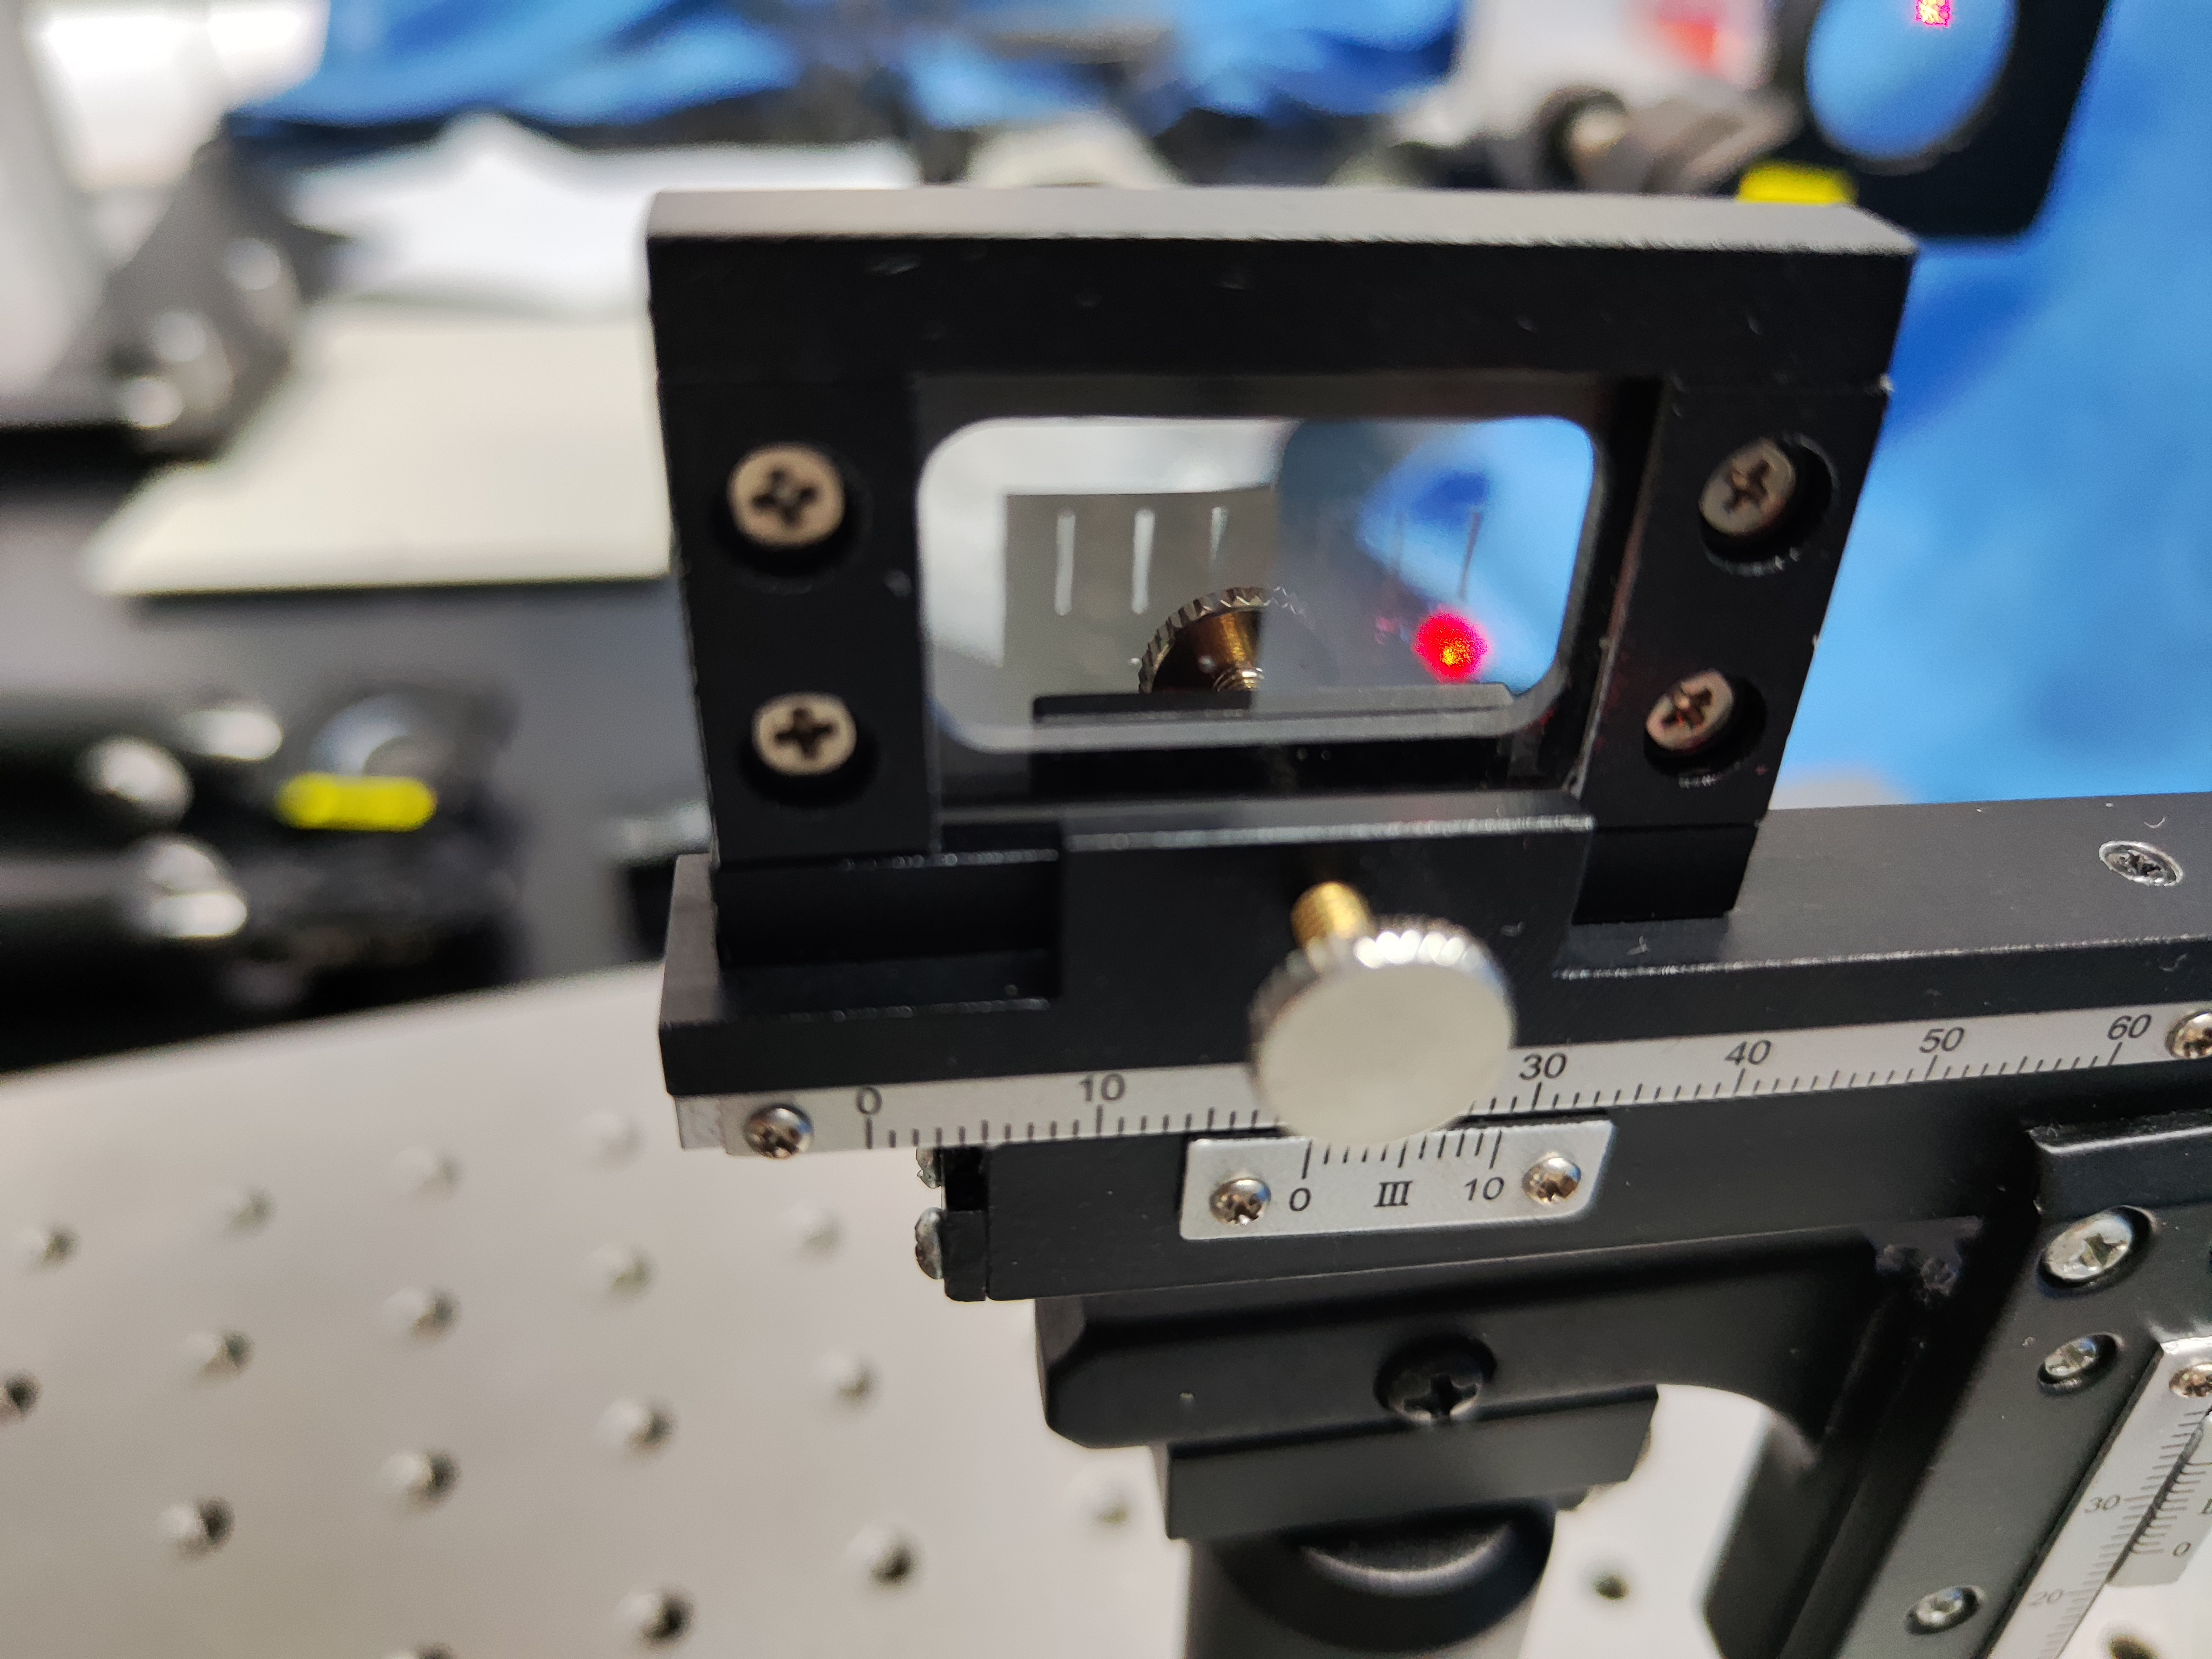
\includegraphics[width=7.5cm]{Fig/3 (5).jpg}}
            \hspace{0.5in}
            \subfigure[]{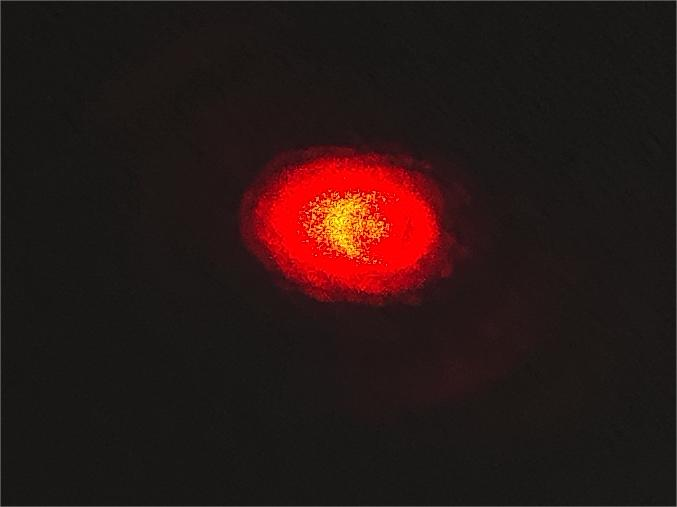
\includegraphics[width=7.5cm]{Fig/3 (6).jpg}}
            \hspace{0.5in}
            \caption{衍射图案}
        \end{figure}
        \begin{figure}[H]
            \centering
            \subfigure[]{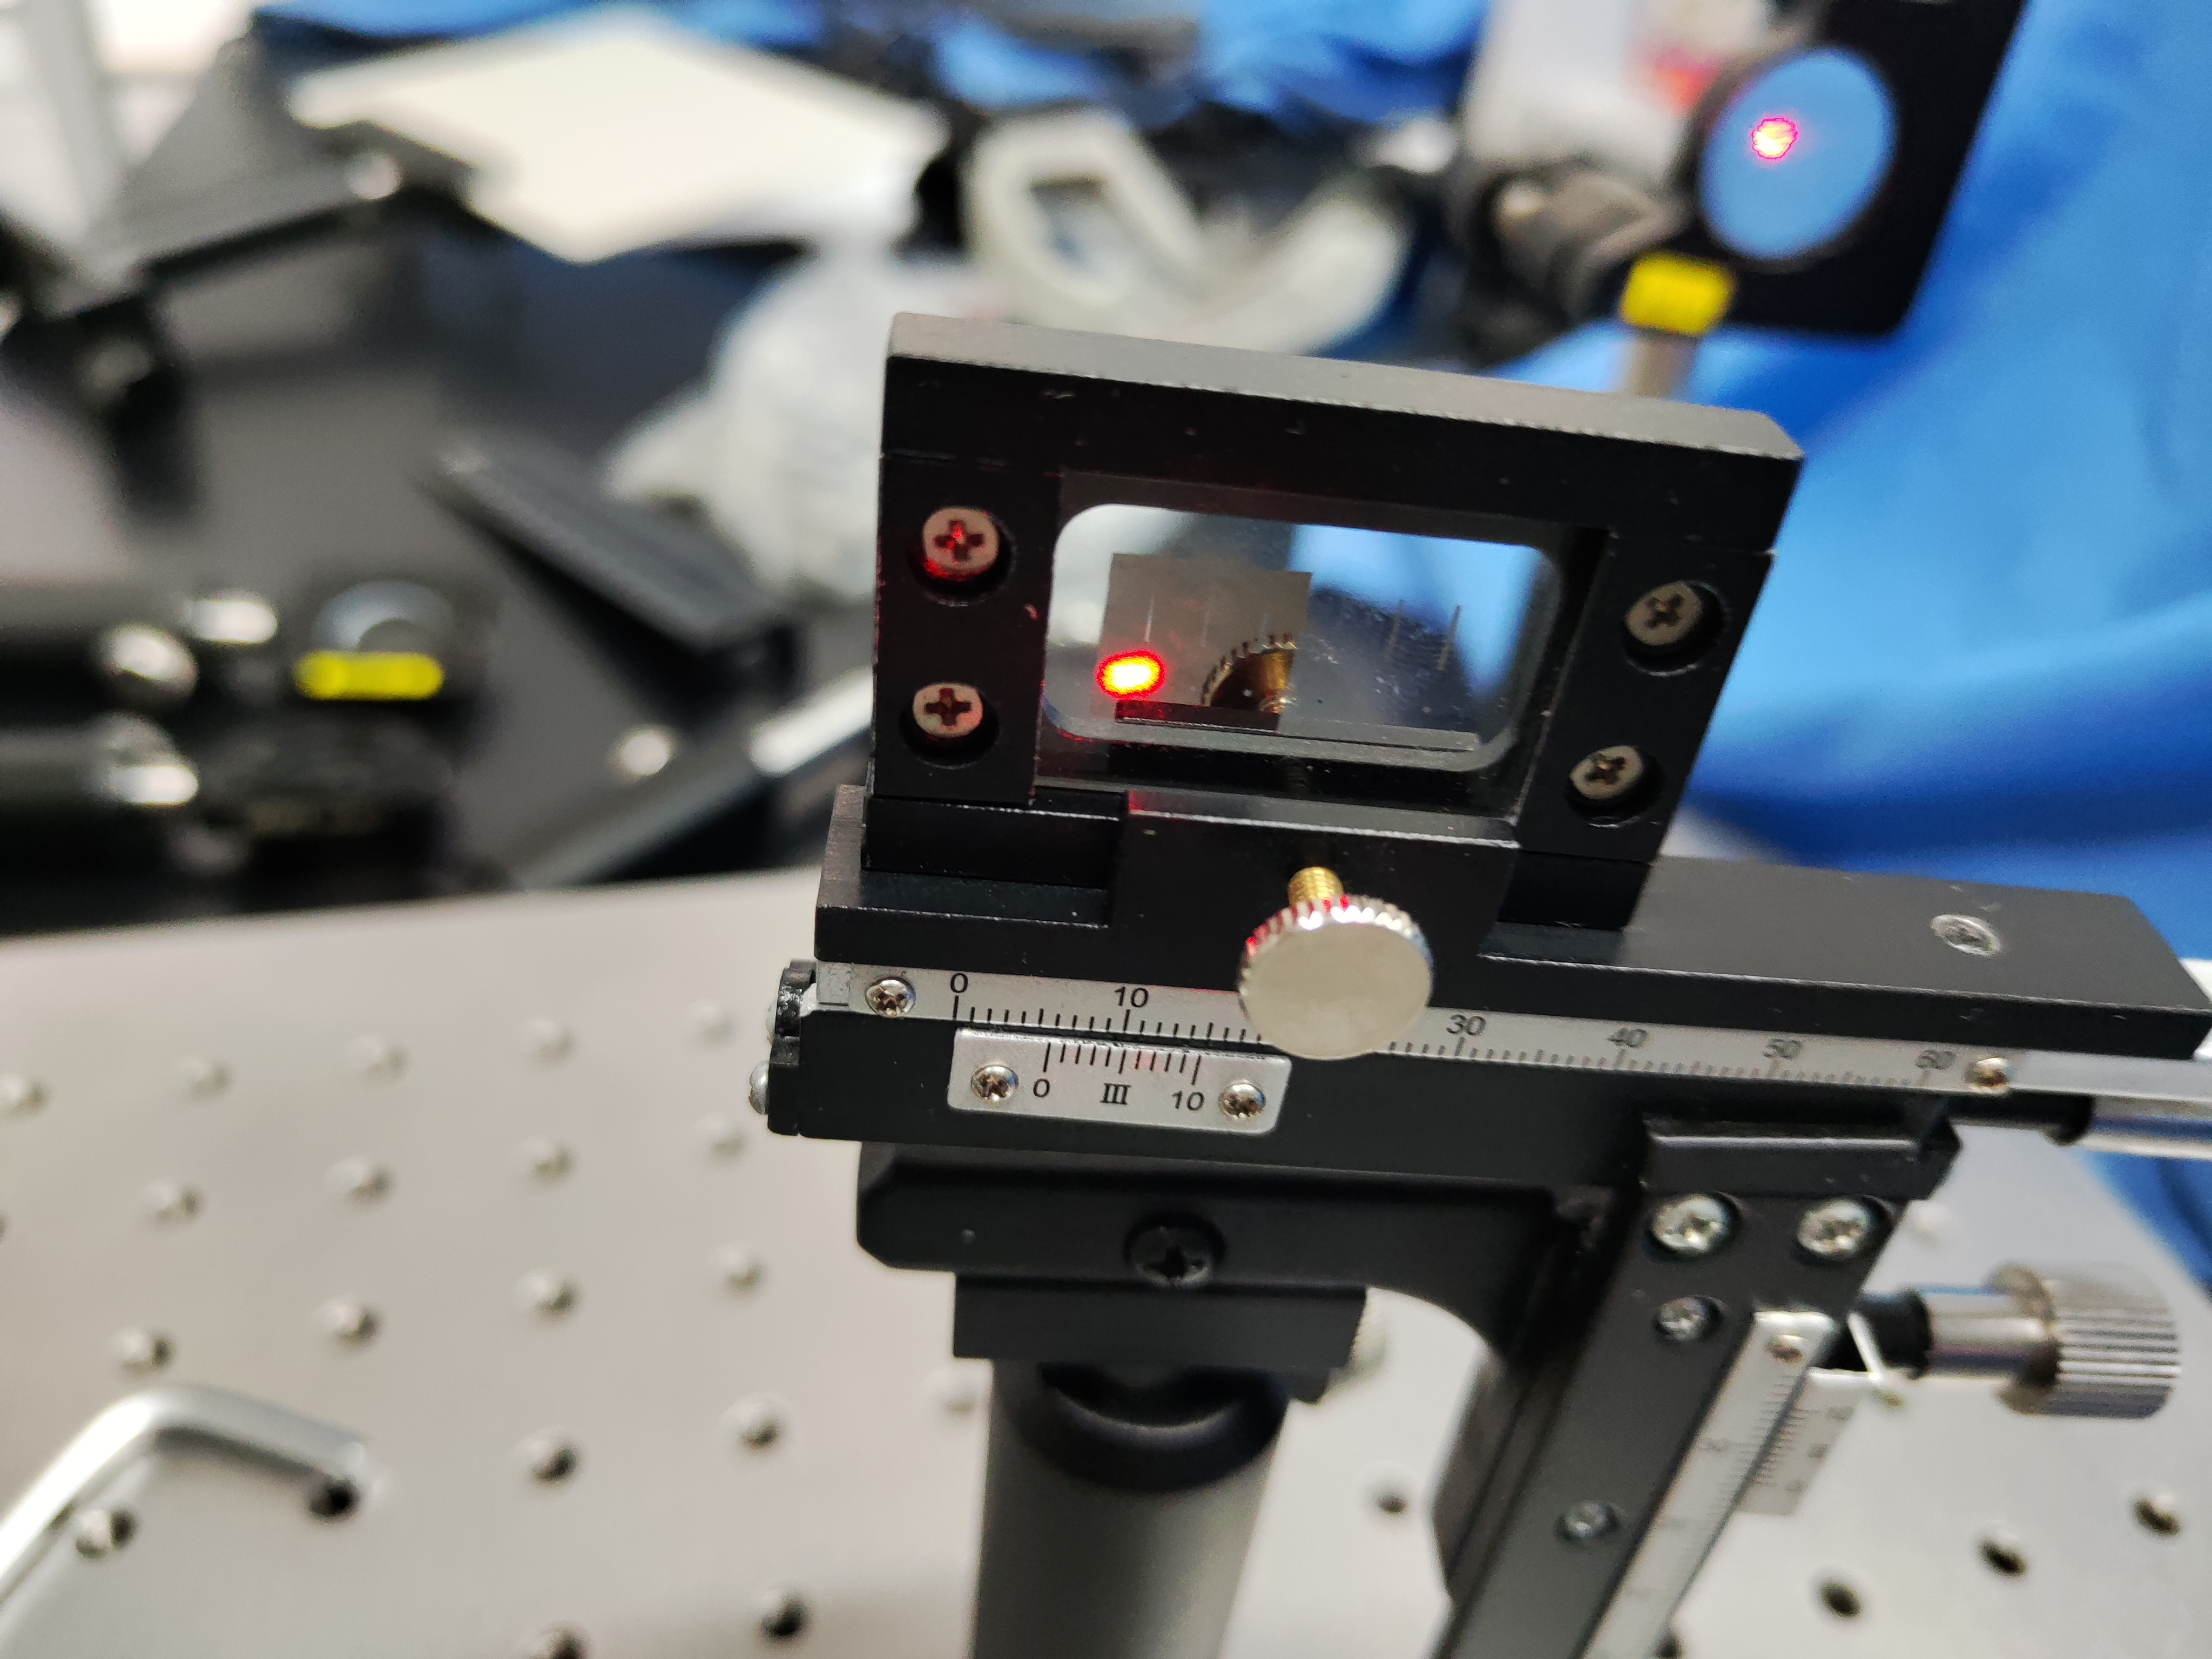
\includegraphics[width=7.5cm]{Fig/3 (7).jpg}}
            \hspace{0.5in}
            \subfigure[]{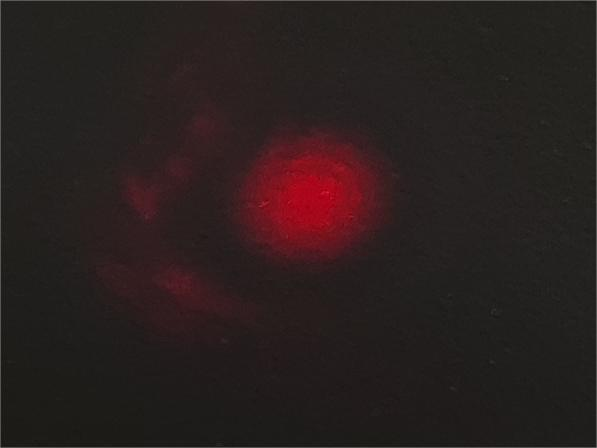
\includegraphics[width=7.5cm]{Fig/3 (8).jpg}}
            \hspace{0.5in}
            \caption{衍射图案}
        \end{figure}
        \begin{figure}[H]
            \centering
            \subfigure[]{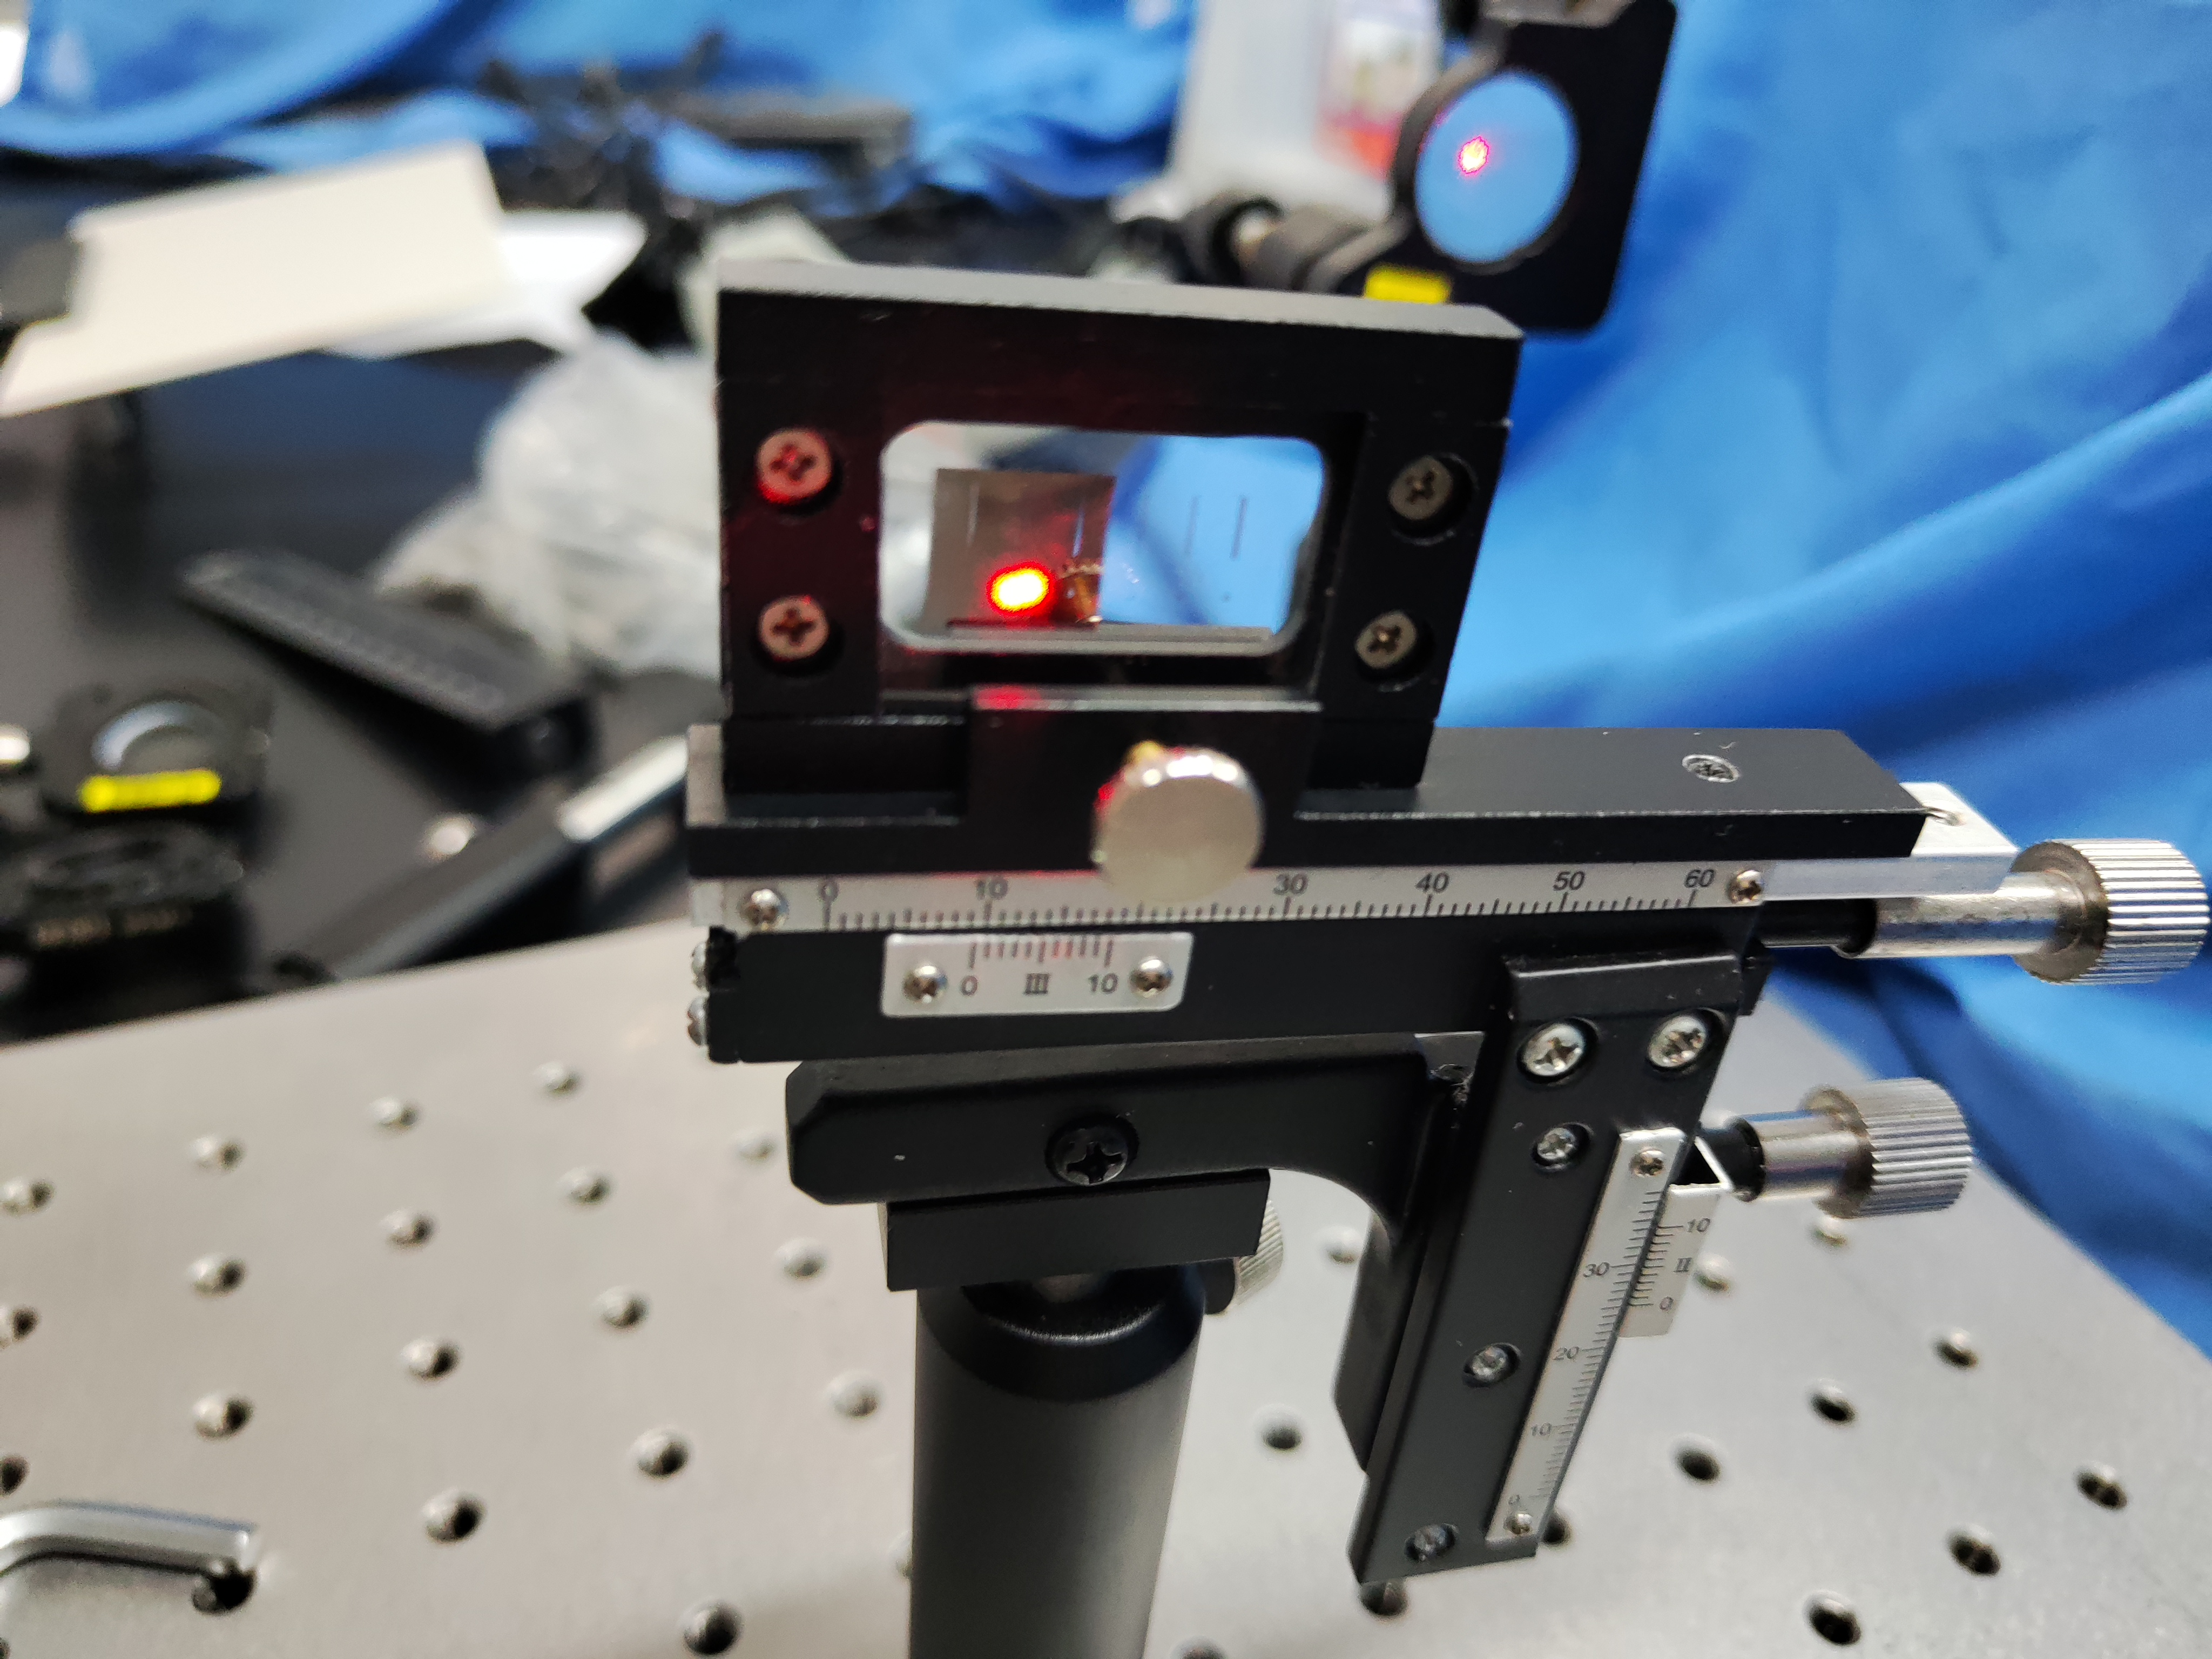
\includegraphics[width=7.5cm]{Fig/3 (9).jpg}}
            \hspace{0.5in}
            \subfigure[]{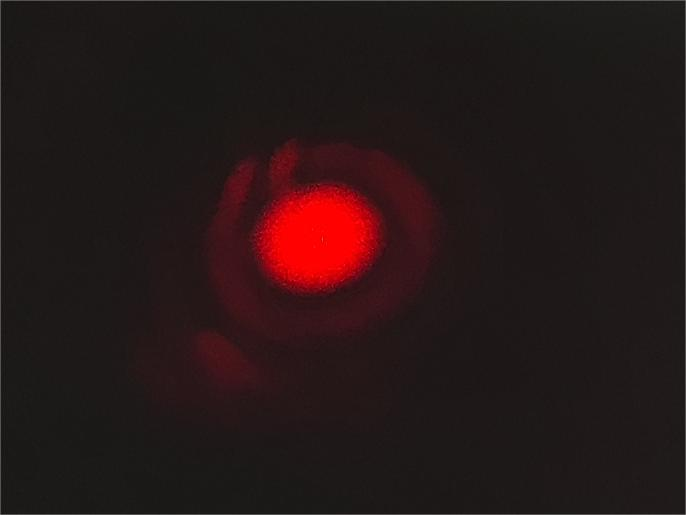
\includegraphics[width=7.5cm]{Fig/3 (10).jpg}}
            \hspace{0.5in}
            \caption{衍射图案}
        \end{figure}
        \begin{figure}[H]
            \centering
            \subfigure[]{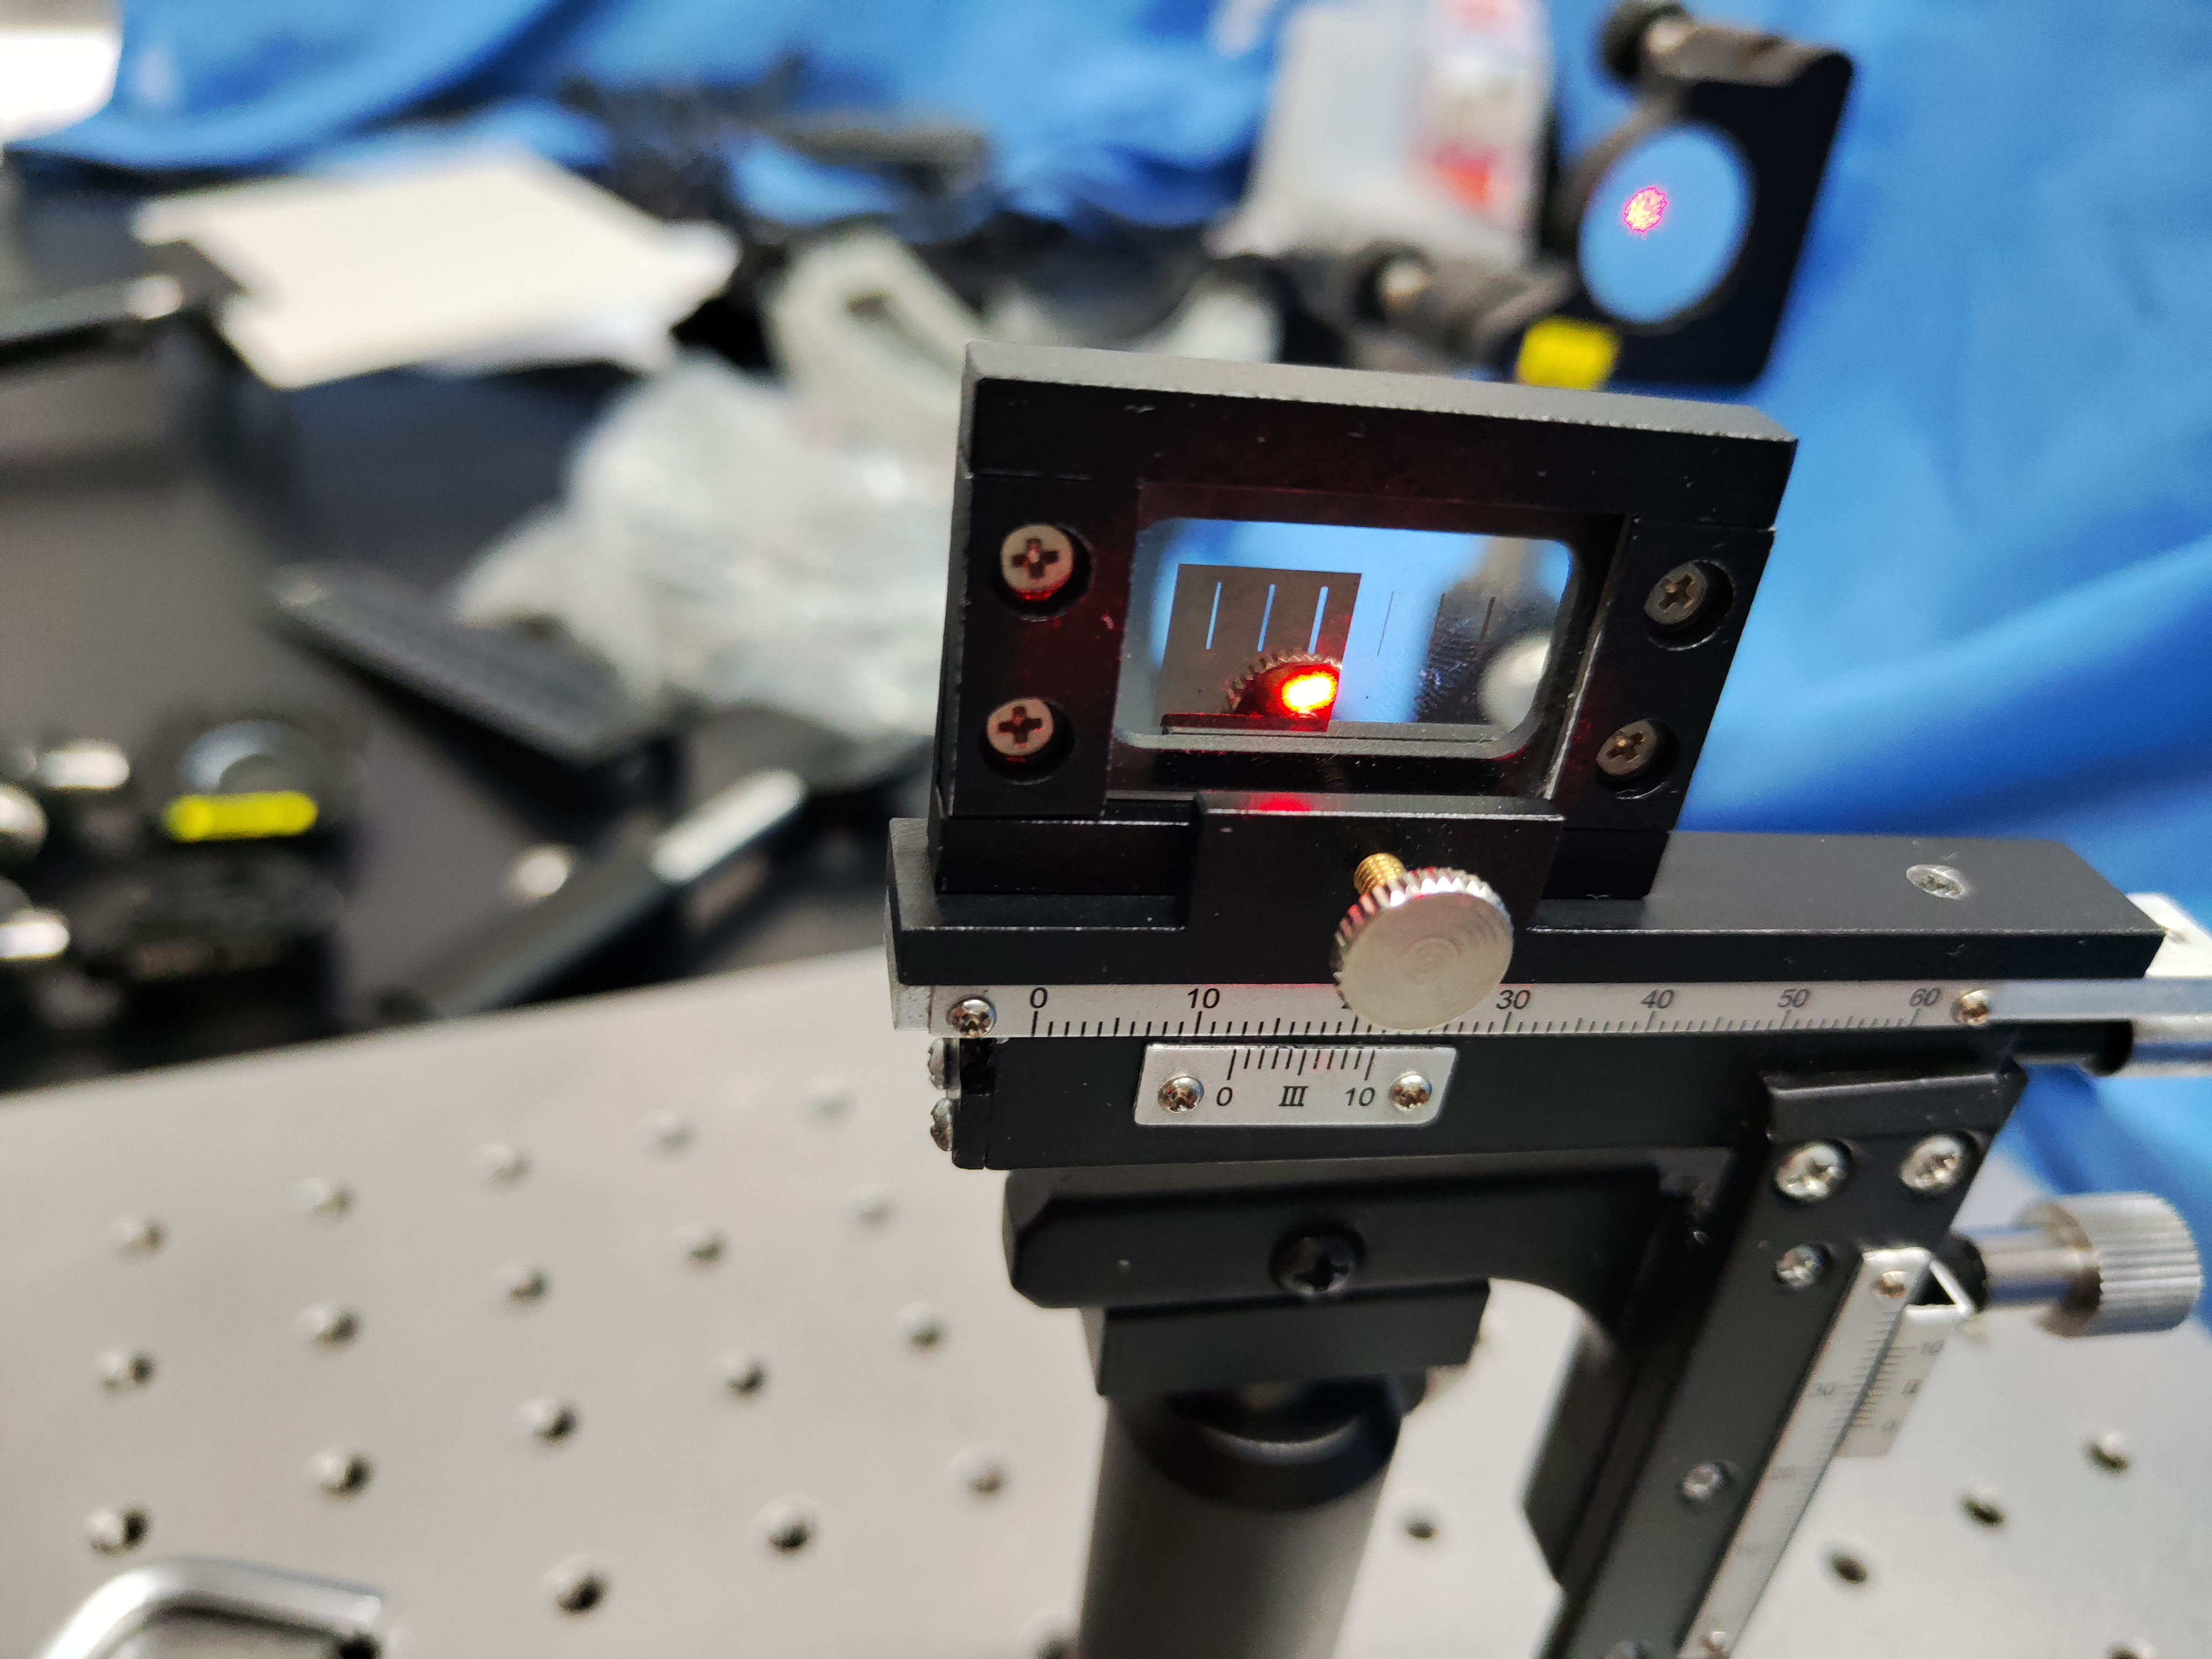
\includegraphics[width=7.5cm]{Fig/3 (11).jpg}}
            \hspace{0.5in}
            \subfigure[]{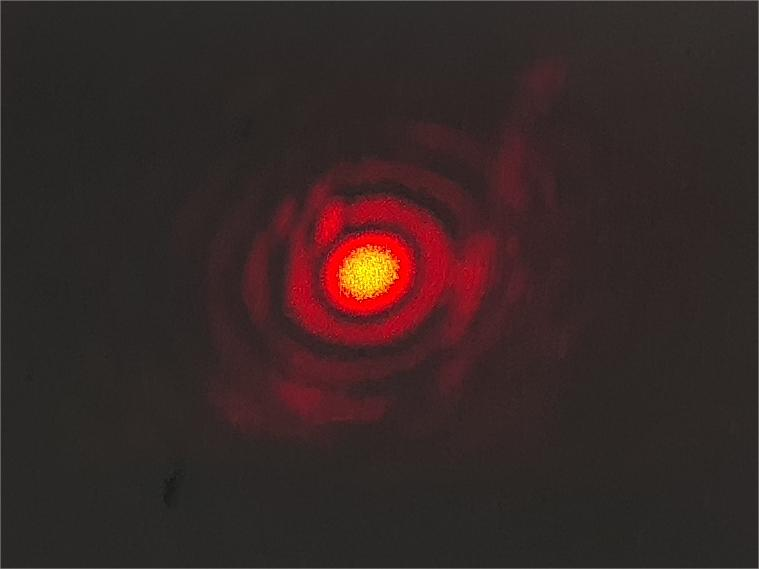
\includegraphics[width=7.5cm]{Fig/3 (12).jpg}}
            \hspace{0.5in}
            \caption{衍射图案}
        \end{figure}
        \begin{figure}[H]
            \centering
            \subfigure[]{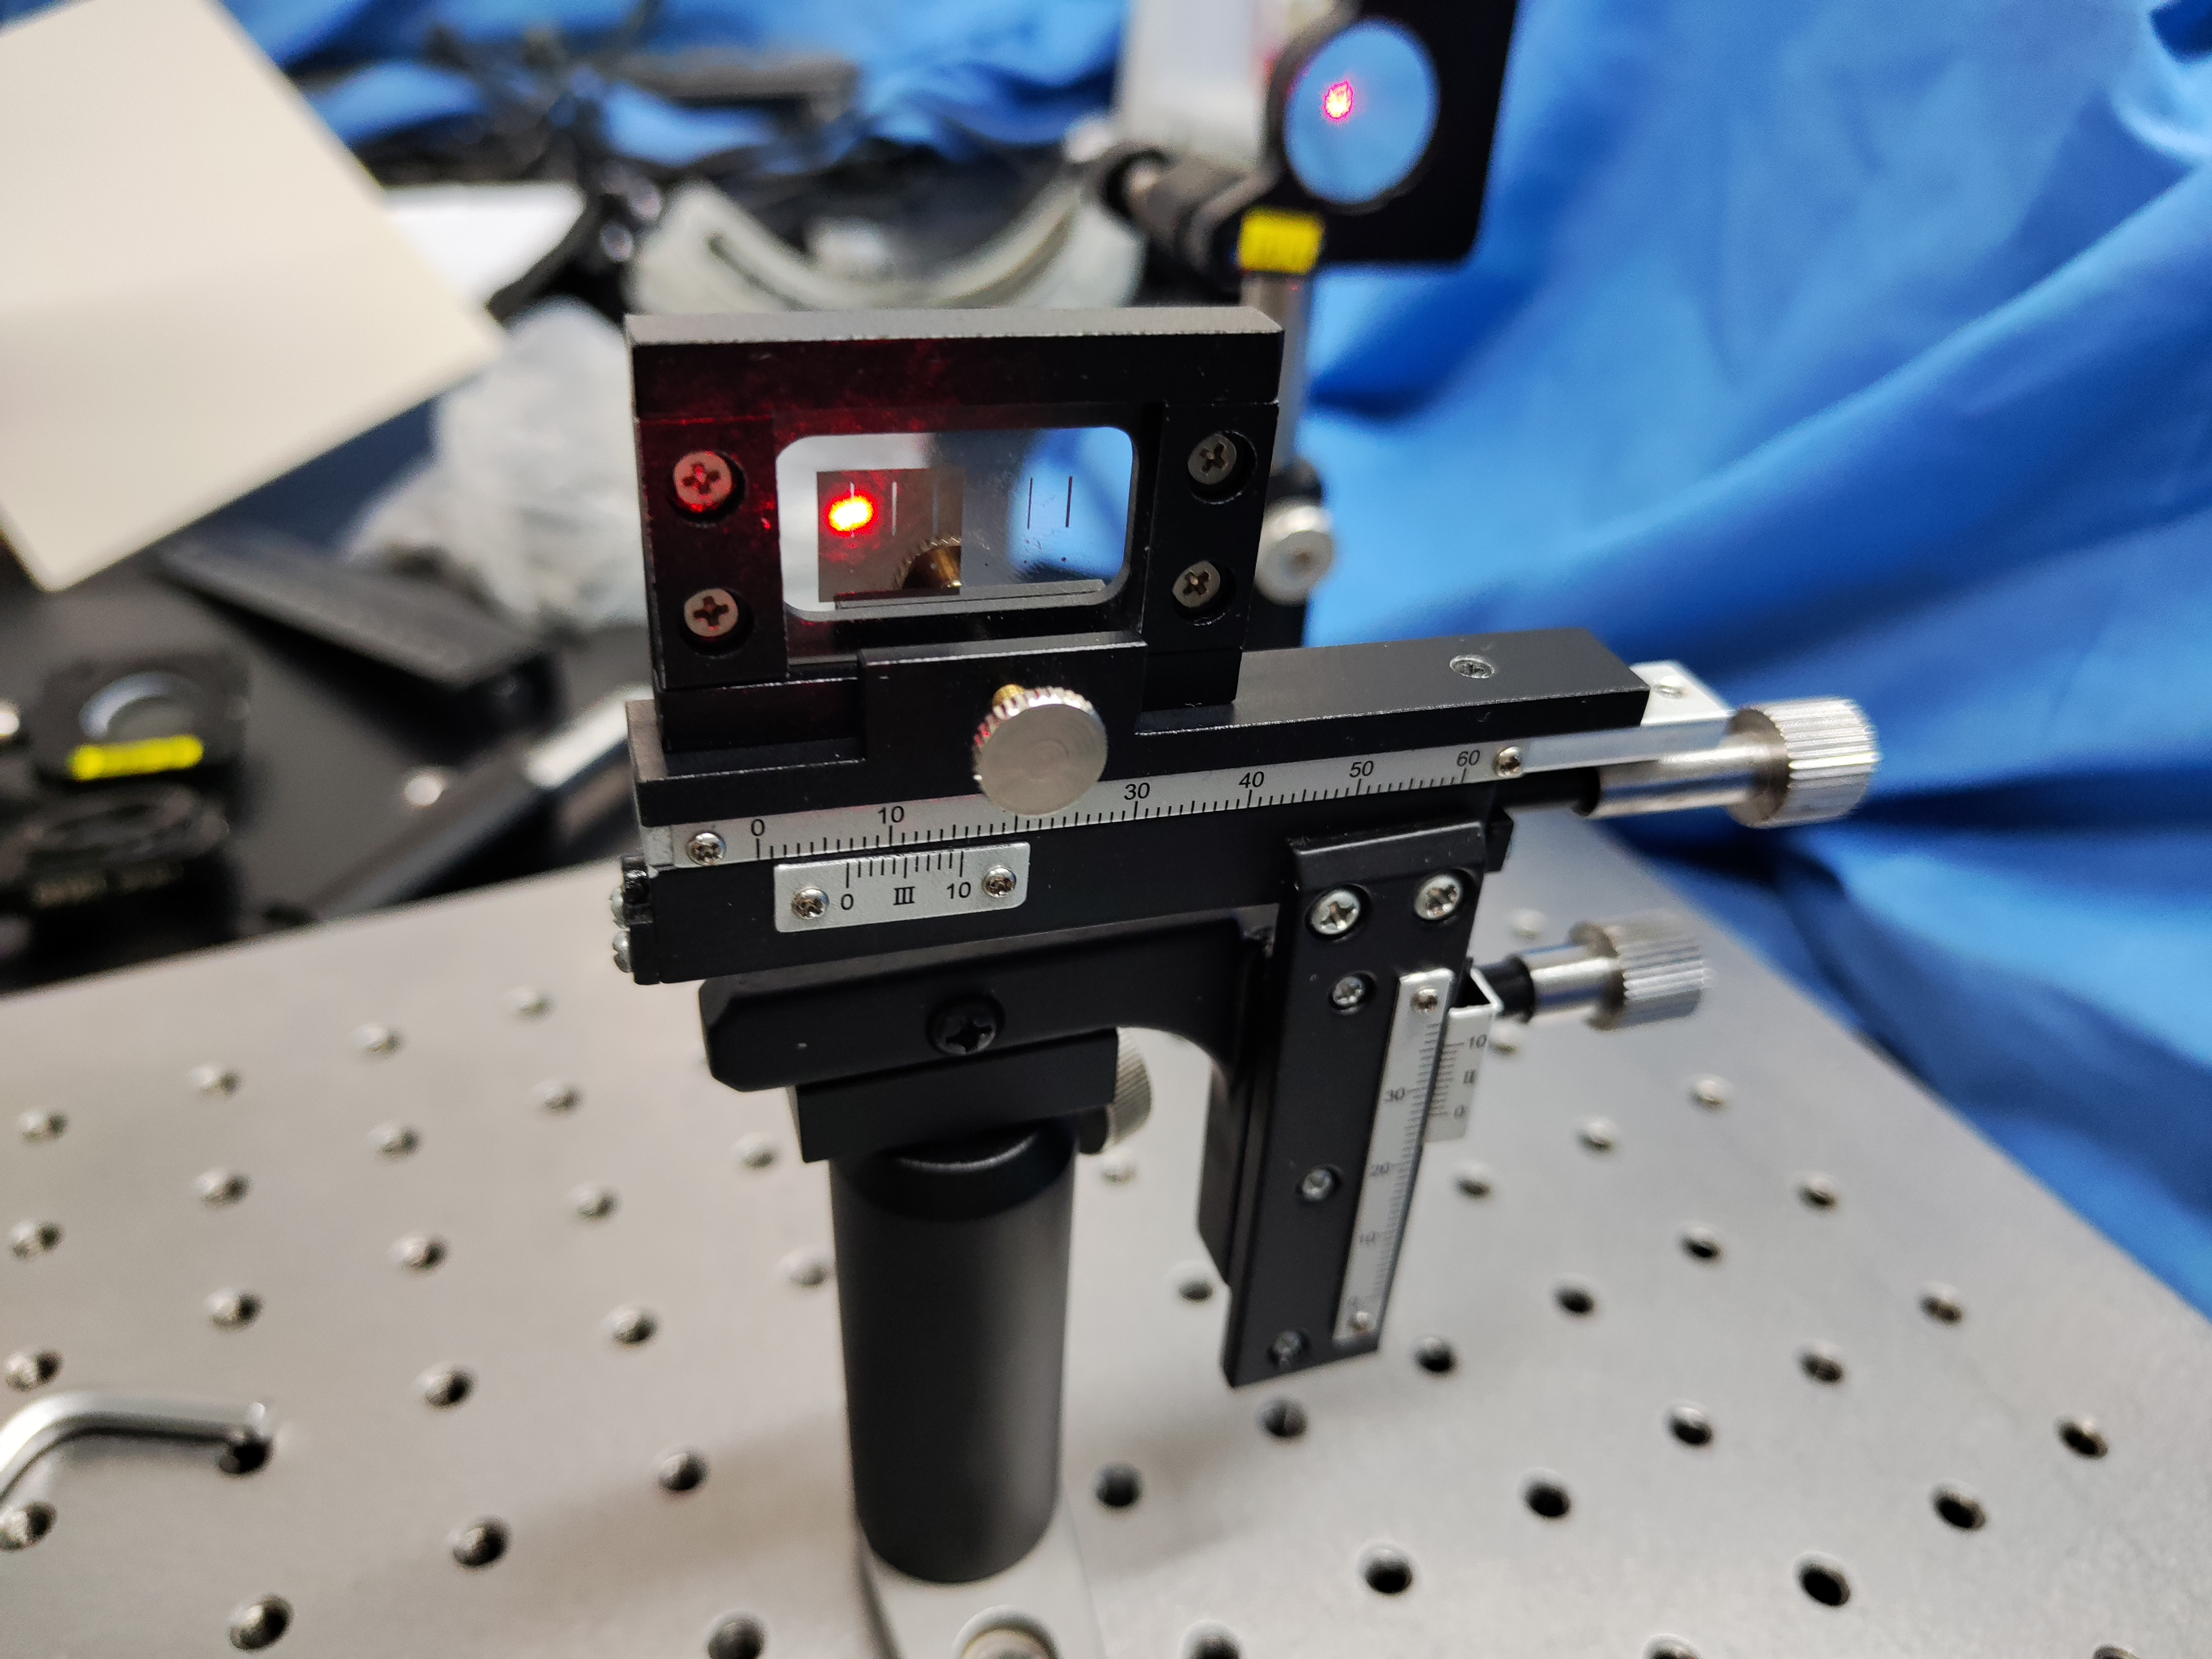
\includegraphics[width=7.5cm]{Fig/3 (13).jpg}}
            \hspace{0.5in}
            \subfigure[]{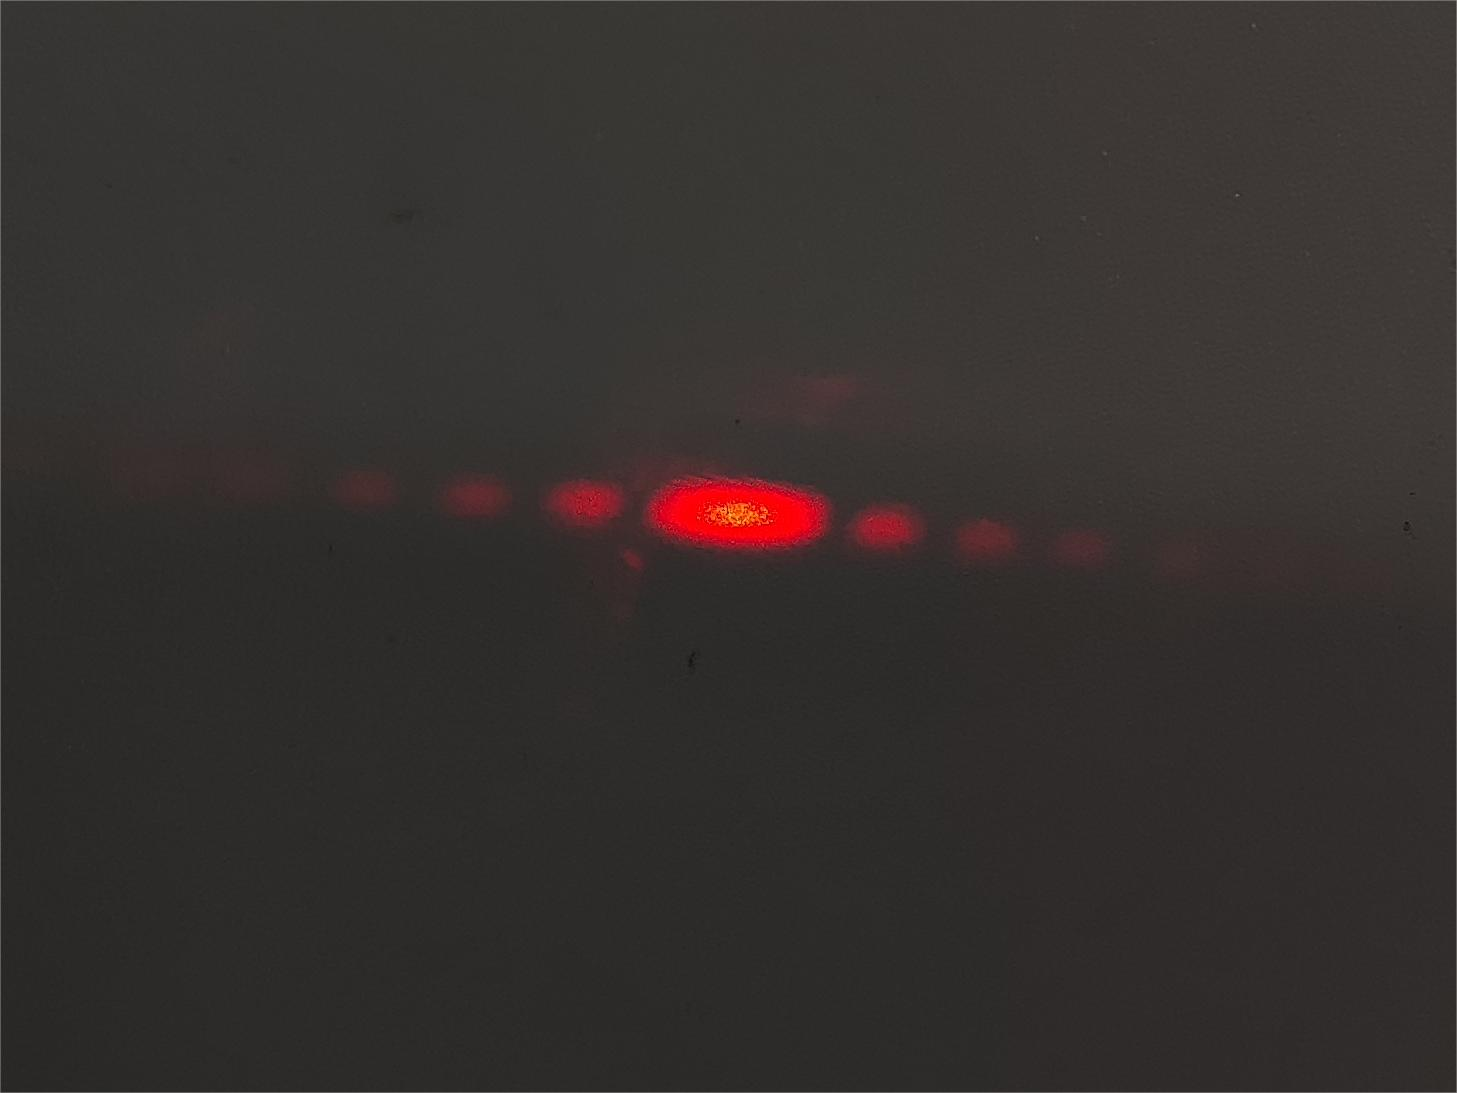
\includegraphics[width=7.5cm]{Fig/3 (14).jpg}}
            \hspace{0.5in}
            \caption{衍射图案}
        \end{figure}
        \begin{figure}[H]
            \centering
            \subfigure[]{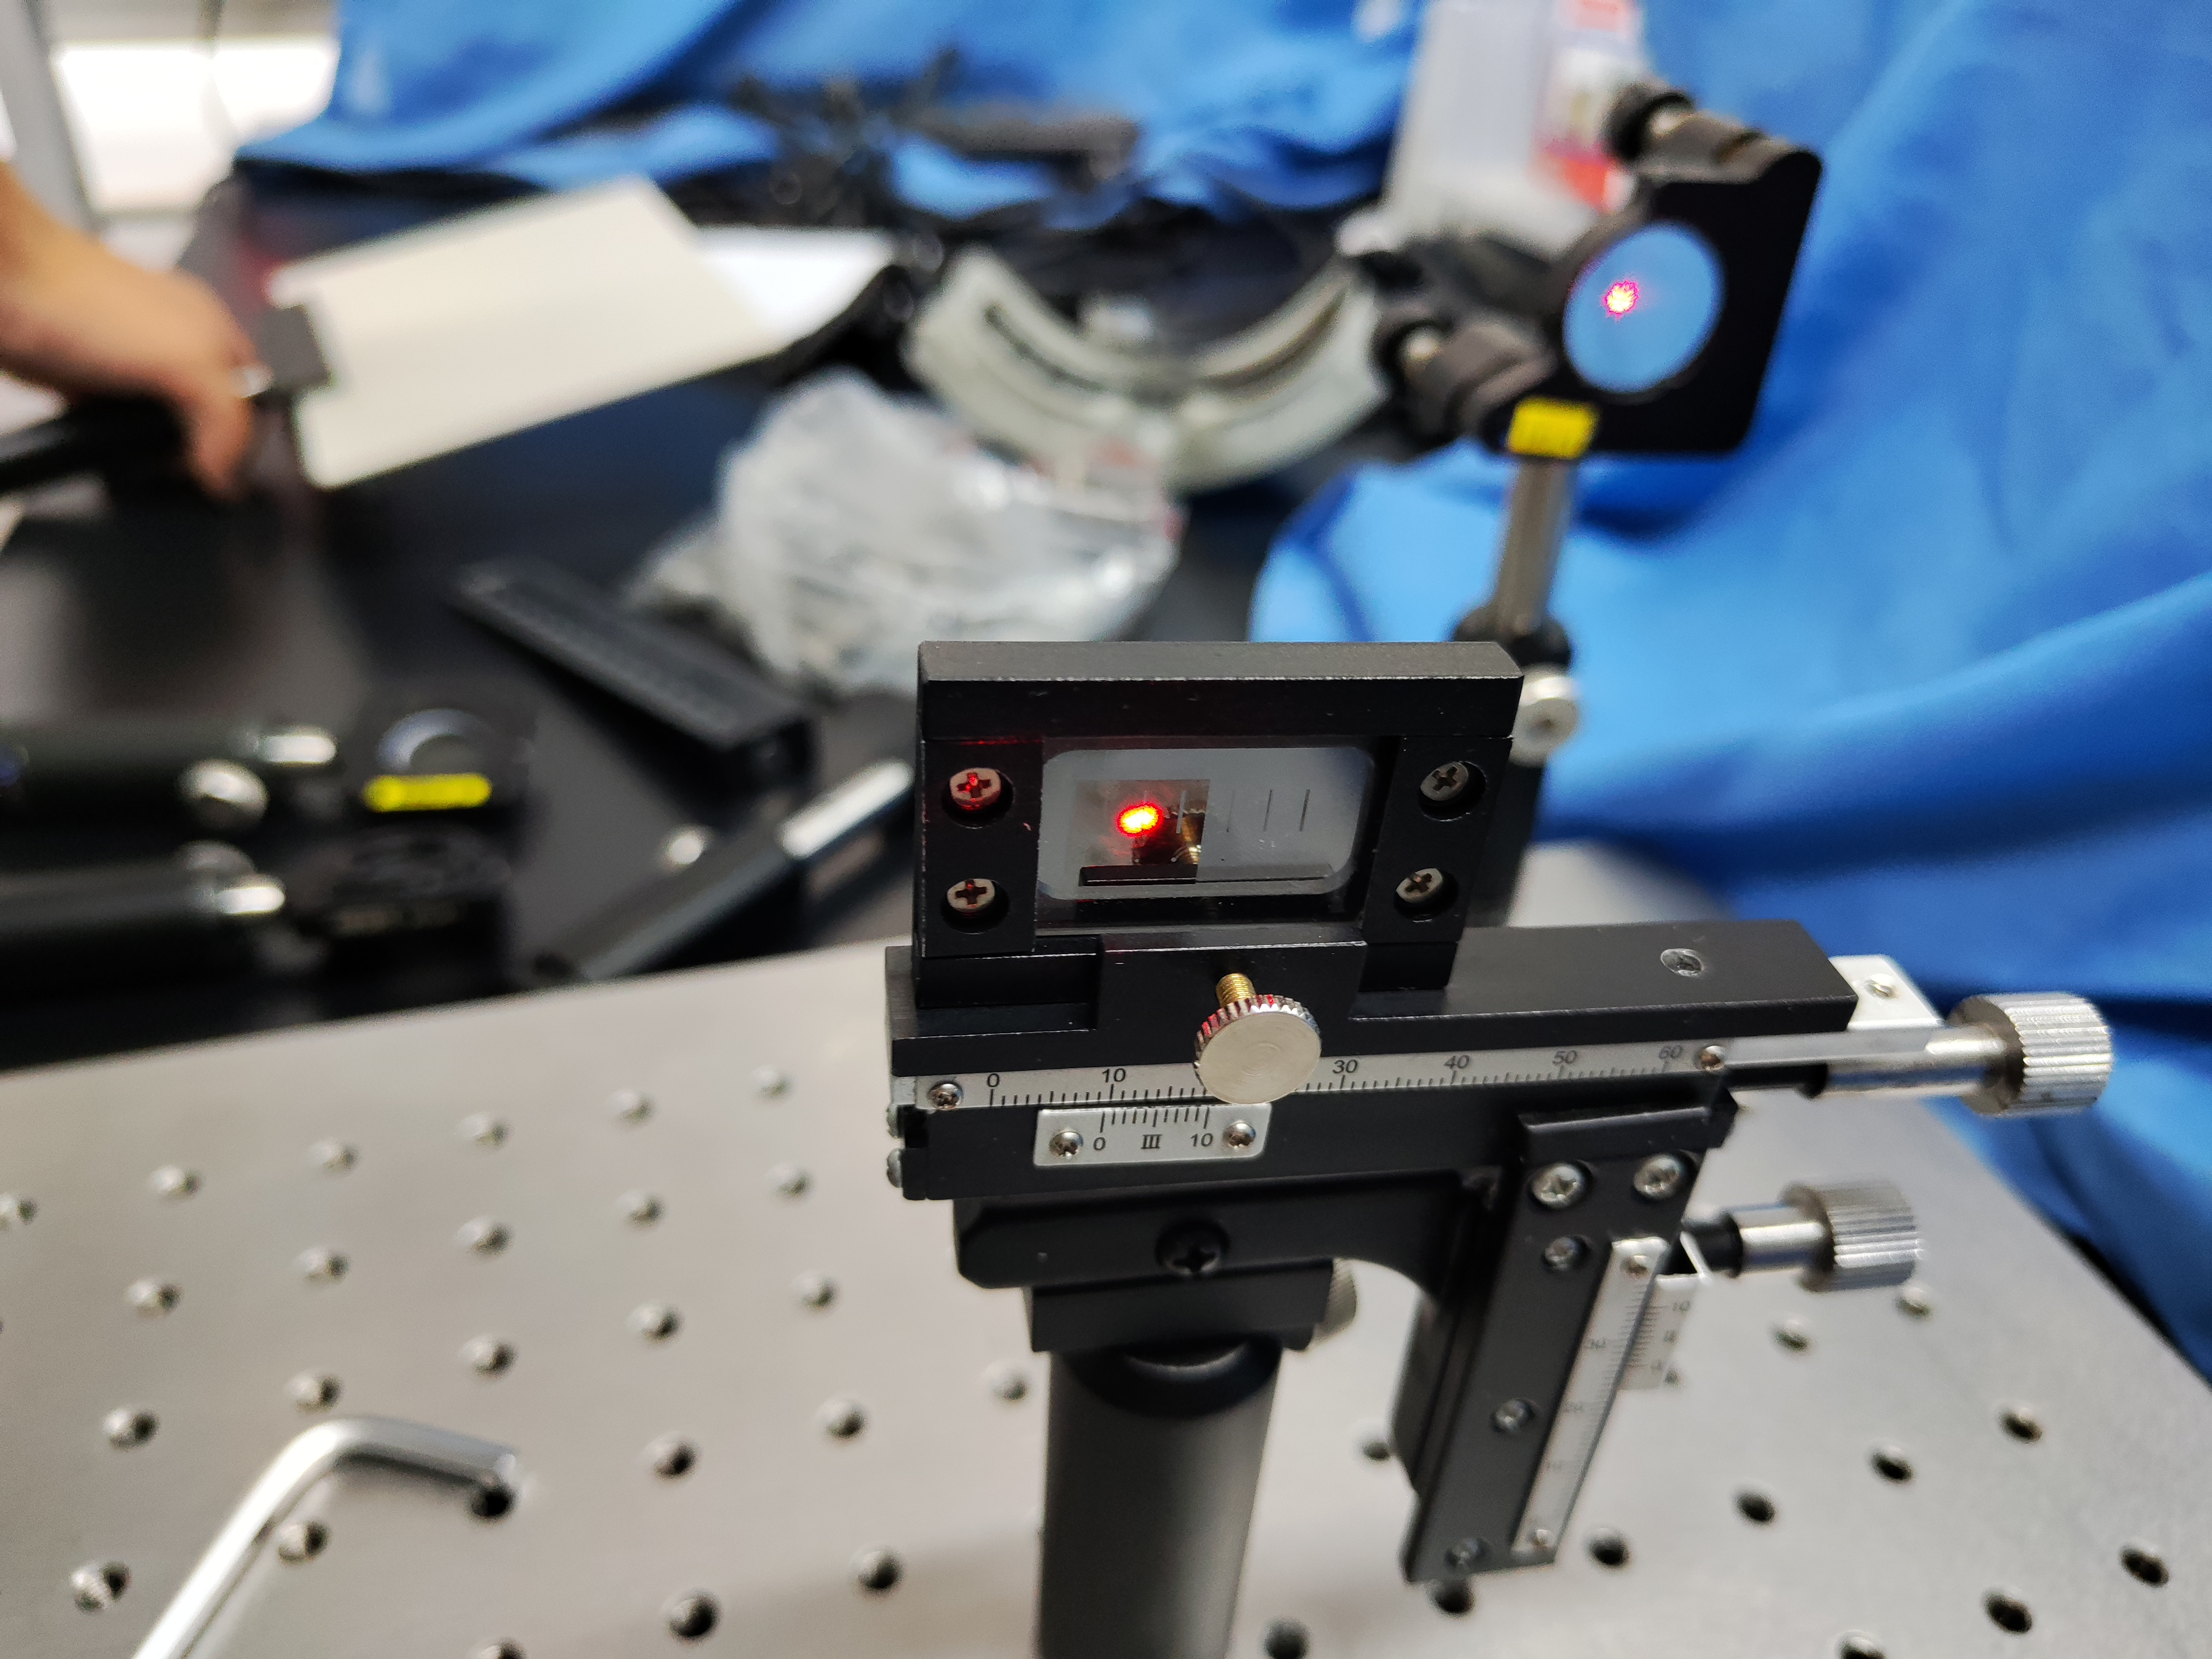
\includegraphics[width=7.5cm]{Fig/3 (15).jpg}}
            \hspace{0.5in}
            \subfigure[]{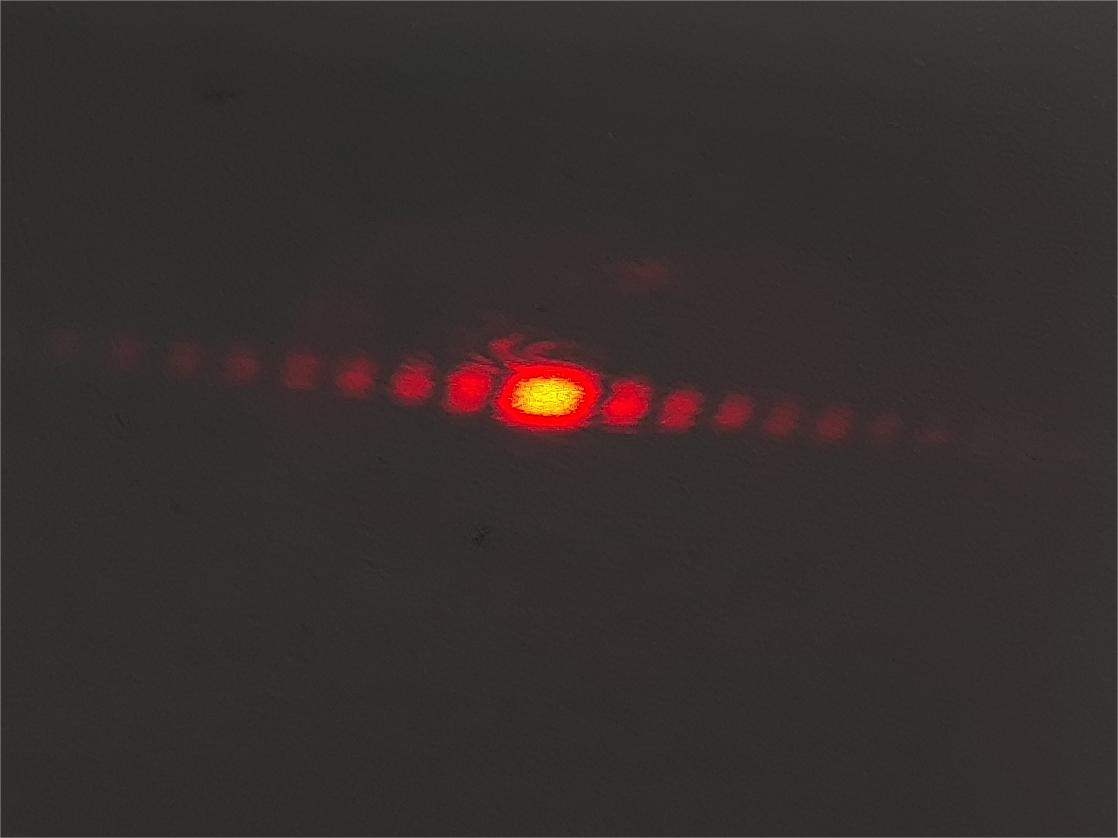
\includegraphics[width=7.5cm]{Fig/3 (16).jpg}}
            \hspace{0.5in}
            \caption{衍射图案}
        \end{figure}
        \begin{figure}[H]
            \centering
            \subfigure[]{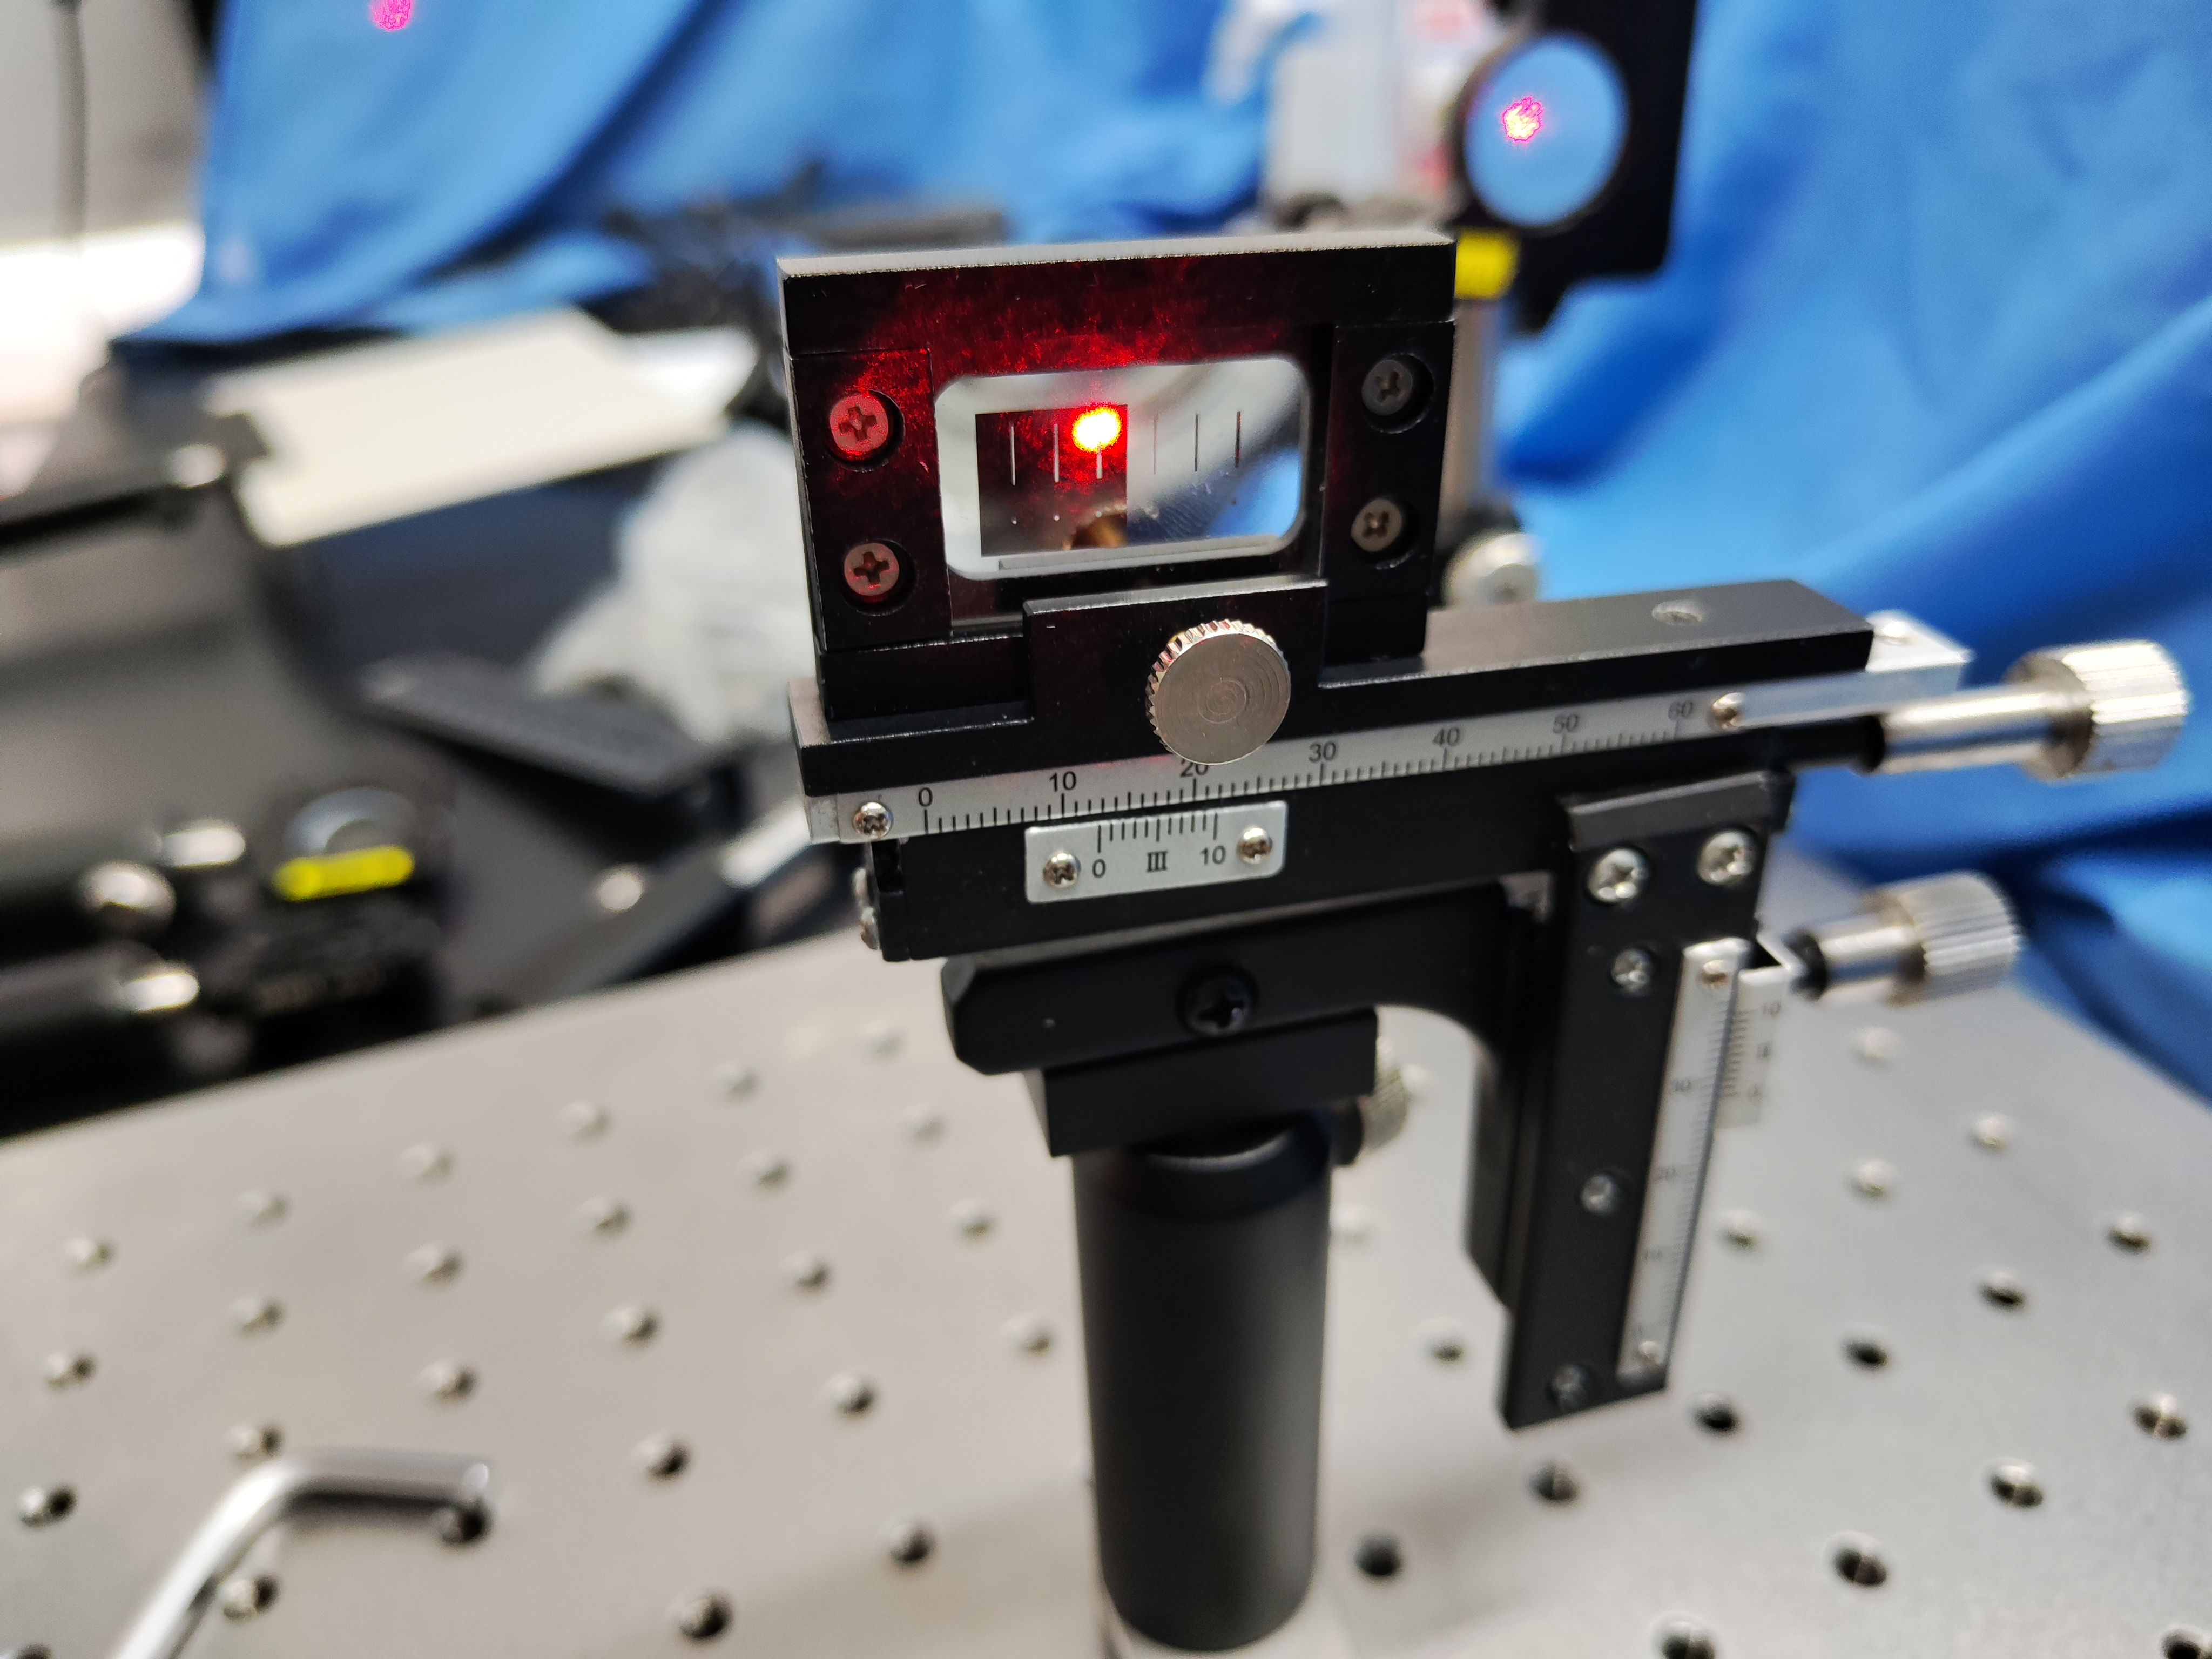
\includegraphics[width=7.5cm]{Fig/3 (17).jpg}}
            \hspace{0.5in}
            \subfigure[]{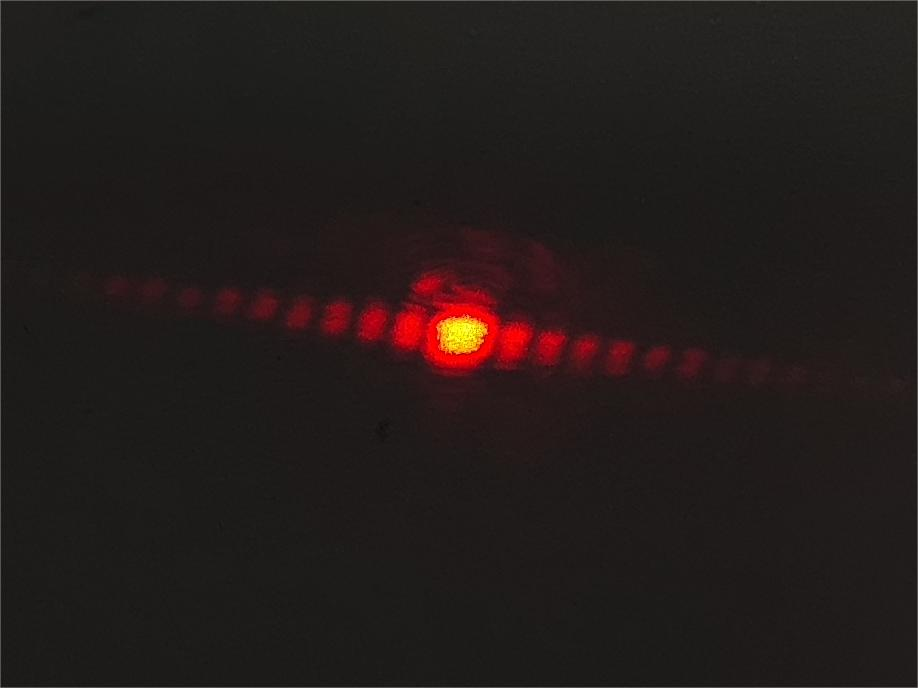
\includegraphics[width=7.5cm]{Fig/3 (18).jpg}}
            \hspace{0.5in}
            \caption{衍射图案}
        \end{figure}
        \begin{figure}[H]
            \centering
            \subfigure[]{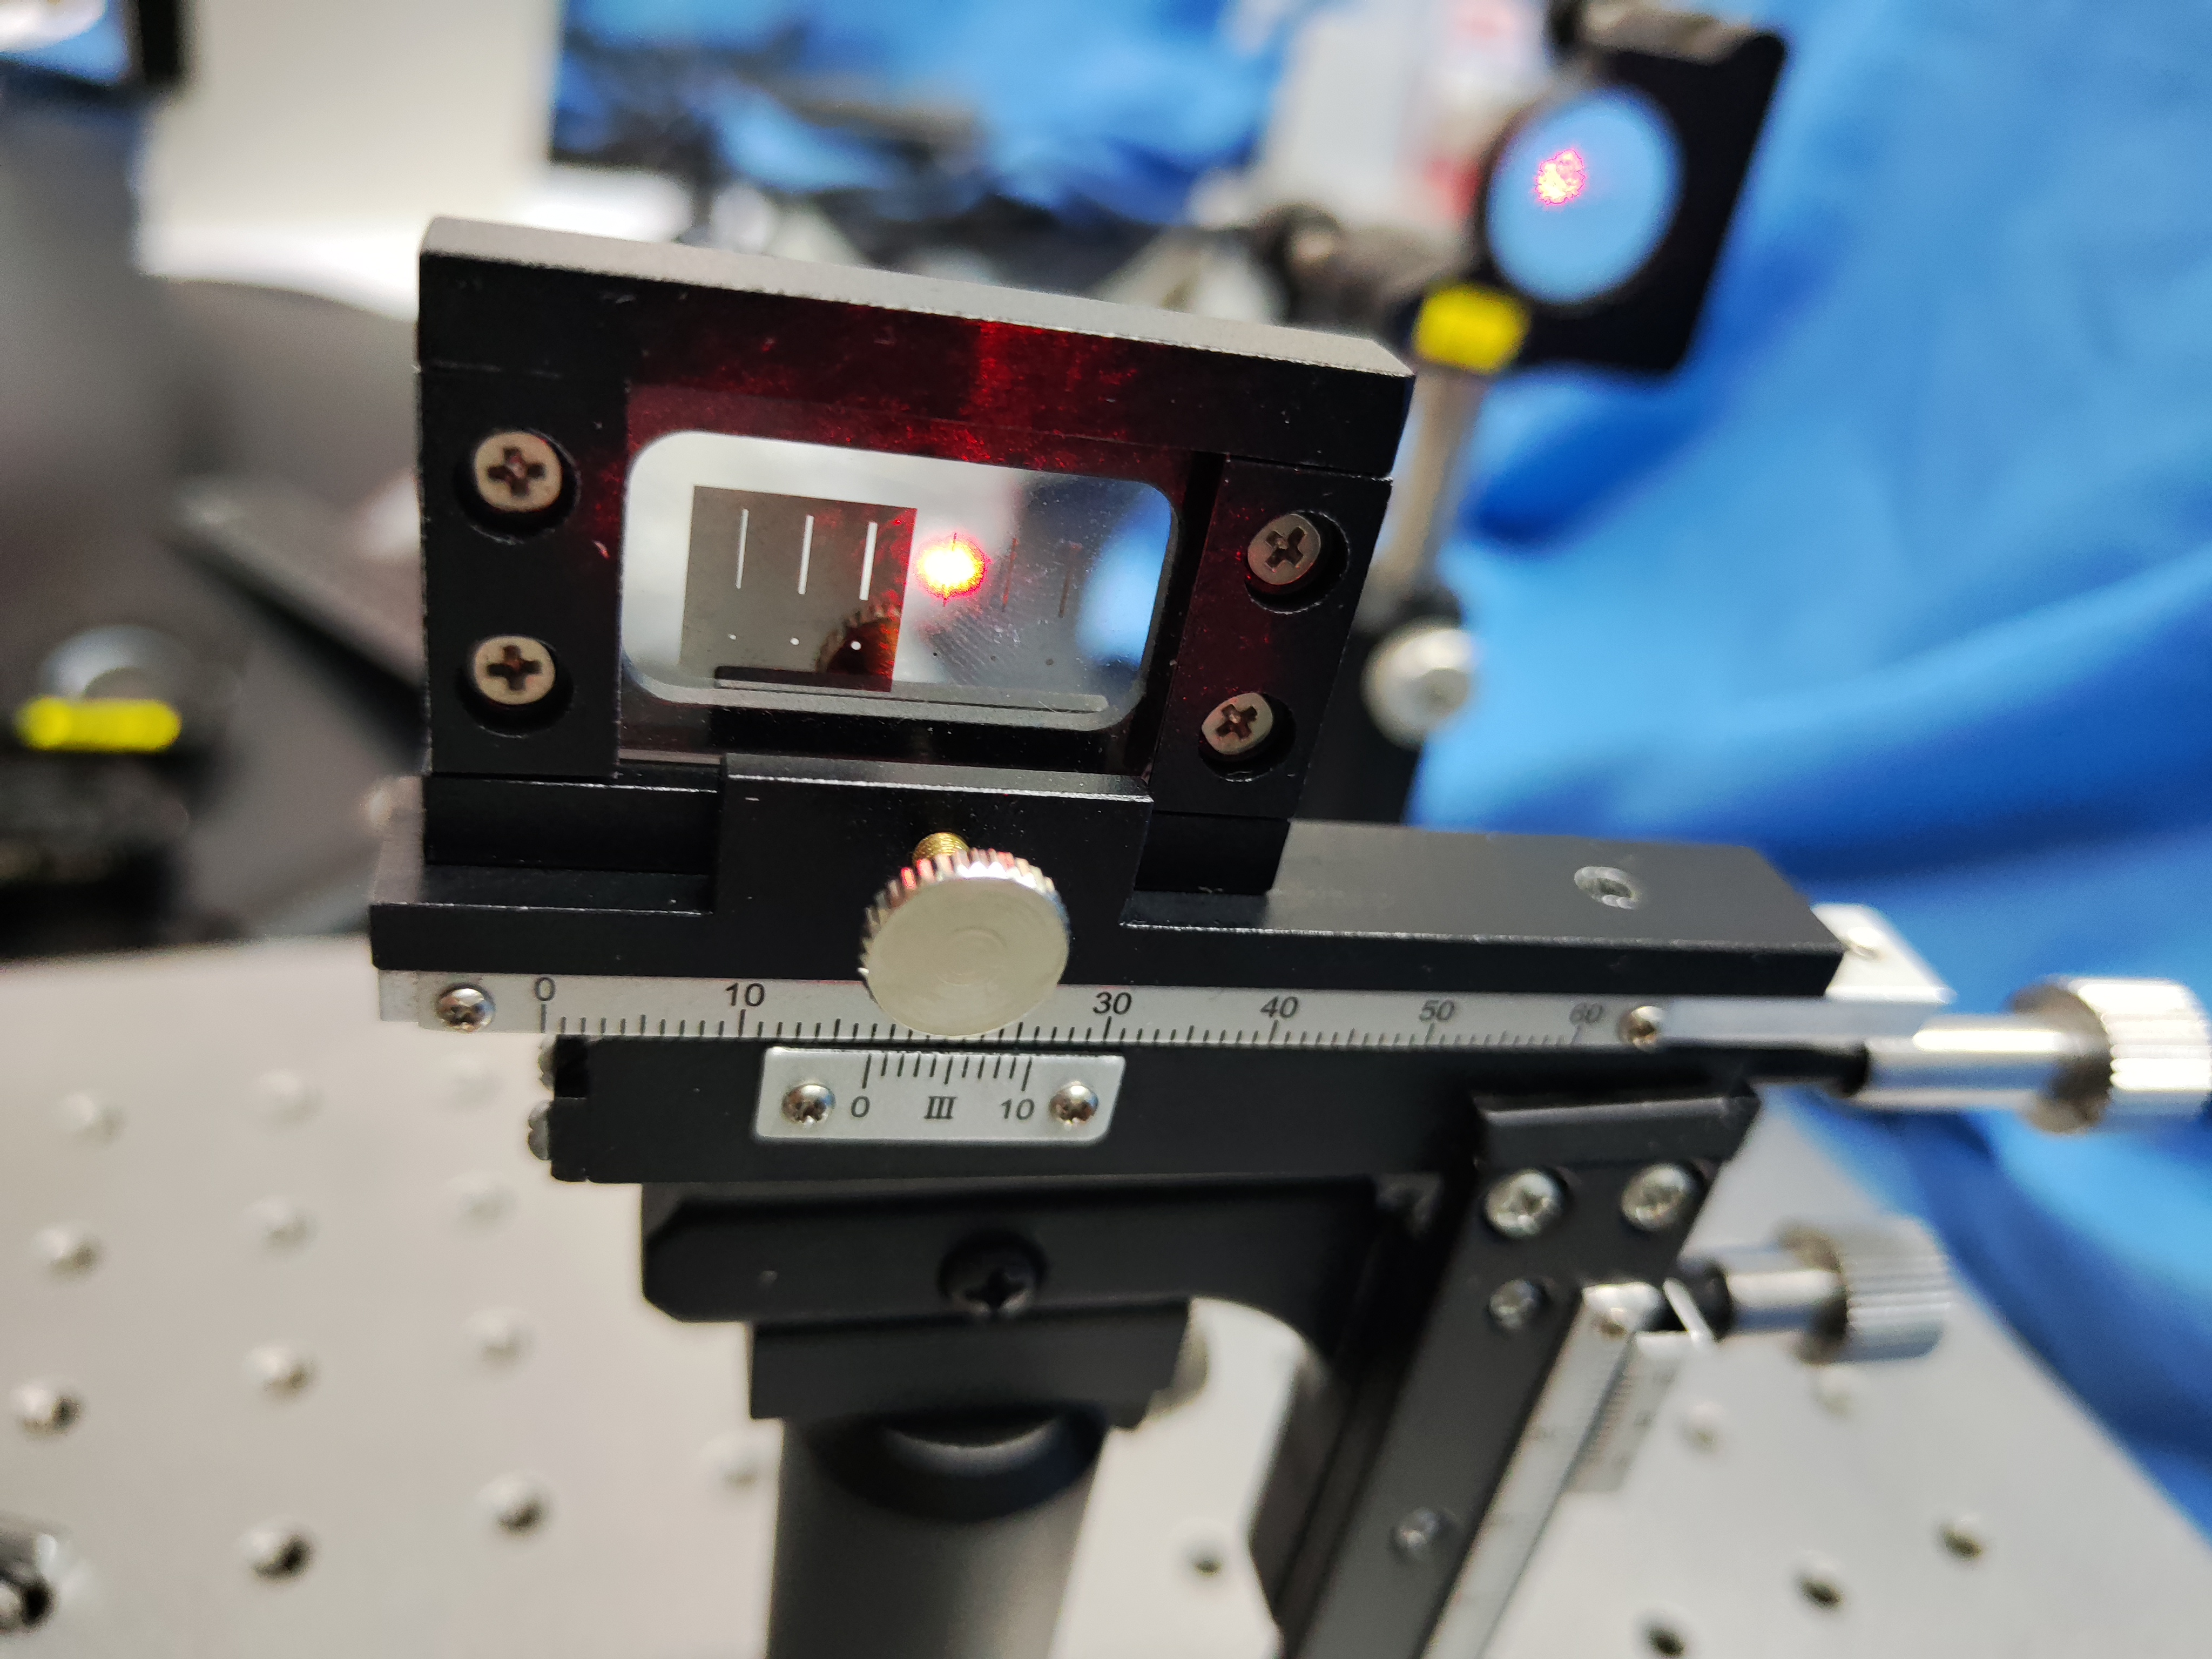
\includegraphics[width=7.5cm]{Fig/3 (19).jpg}}
            \hspace{0.5in}
            \subfigure[]{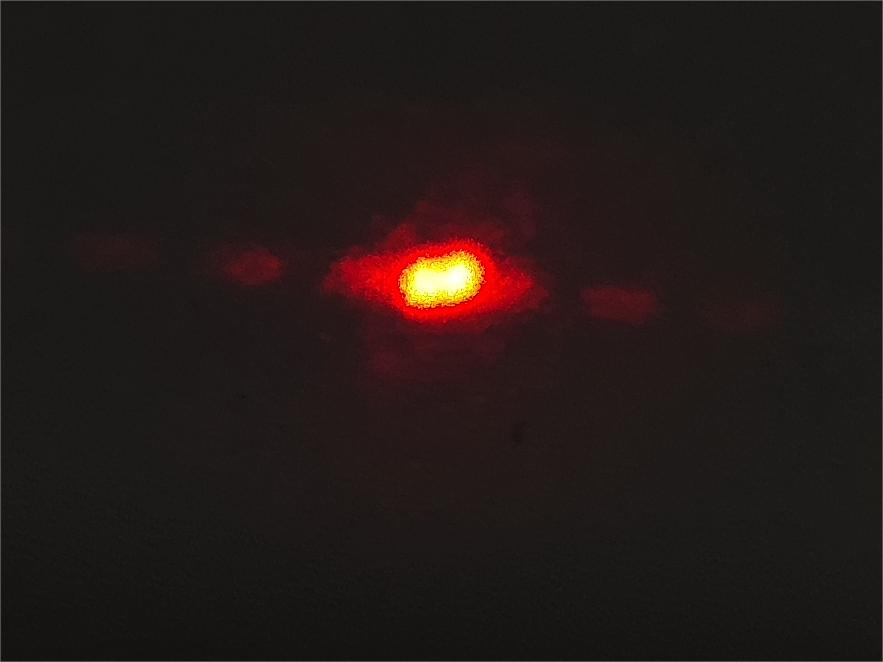
\includegraphics[width=7.5cm]{Fig/3 (20).jpg}}
            \hspace{0.5in}
            \caption{衍射图案}
        \end{figure}
        \begin{figure}[H]
            \centering
            \subfigure[]{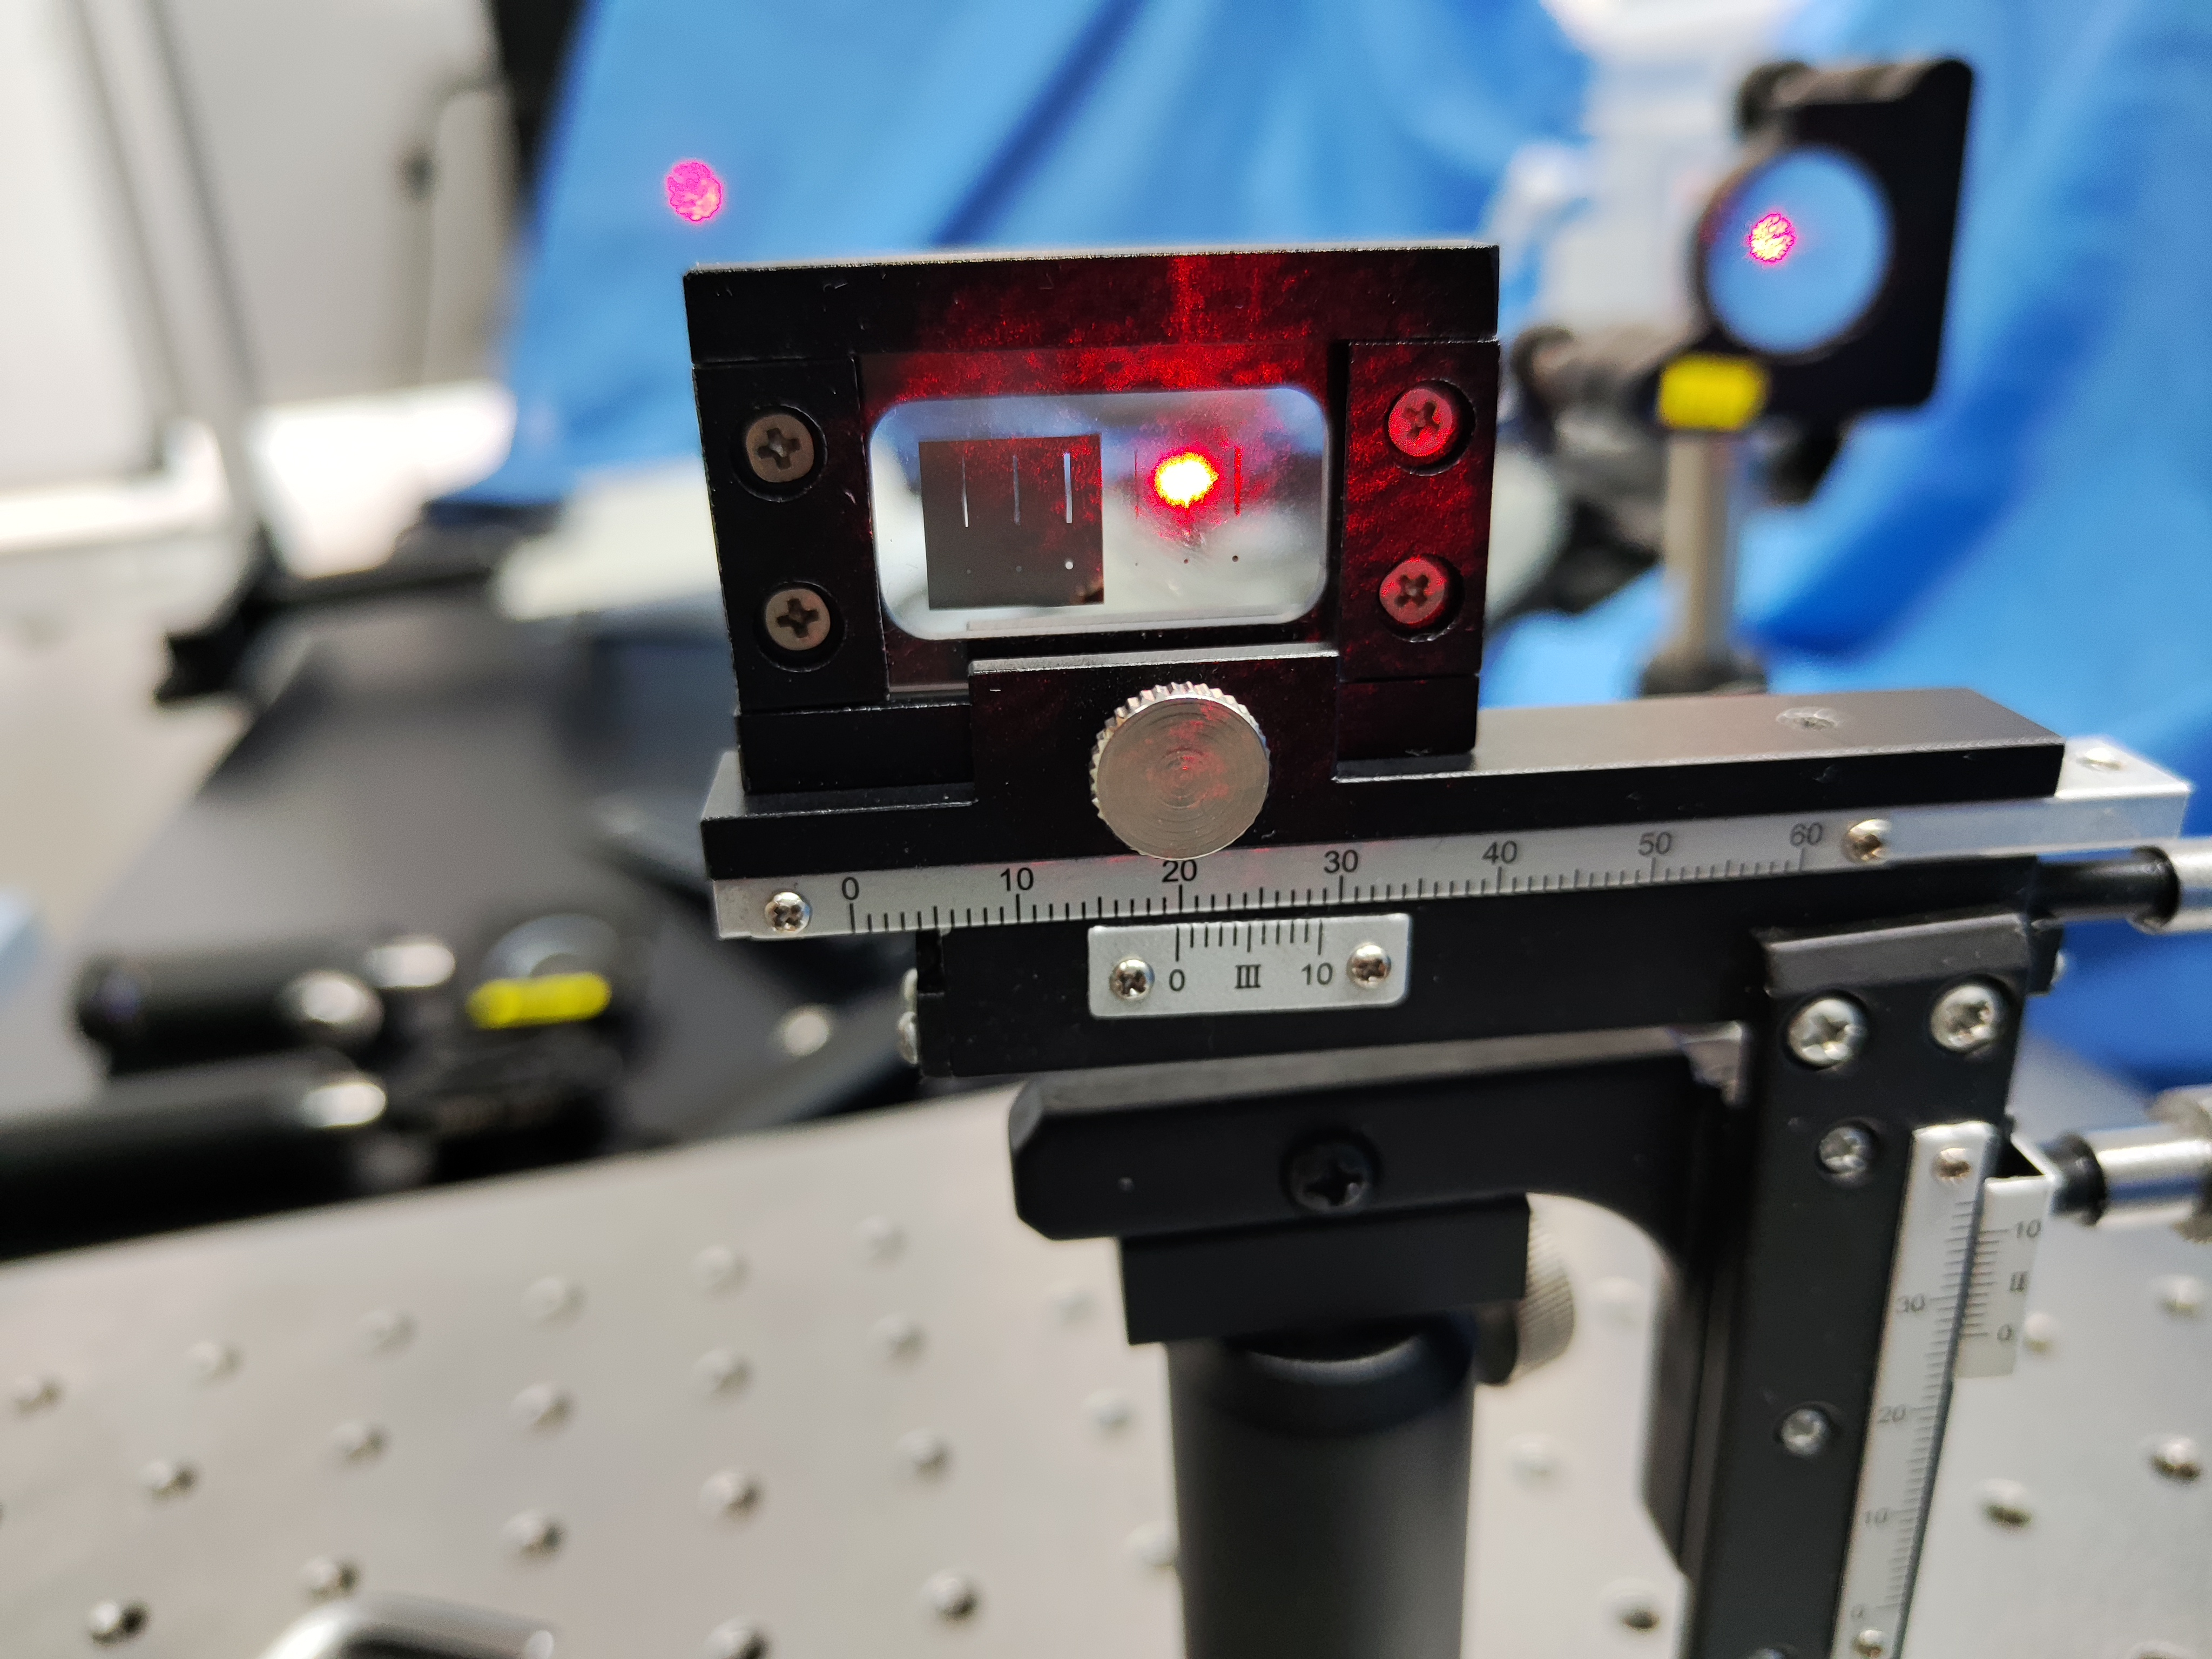
\includegraphics[width=7.5cm]{Fig/3 (21).jpg}}
            \hspace{0.5in}
            \subfigure[]{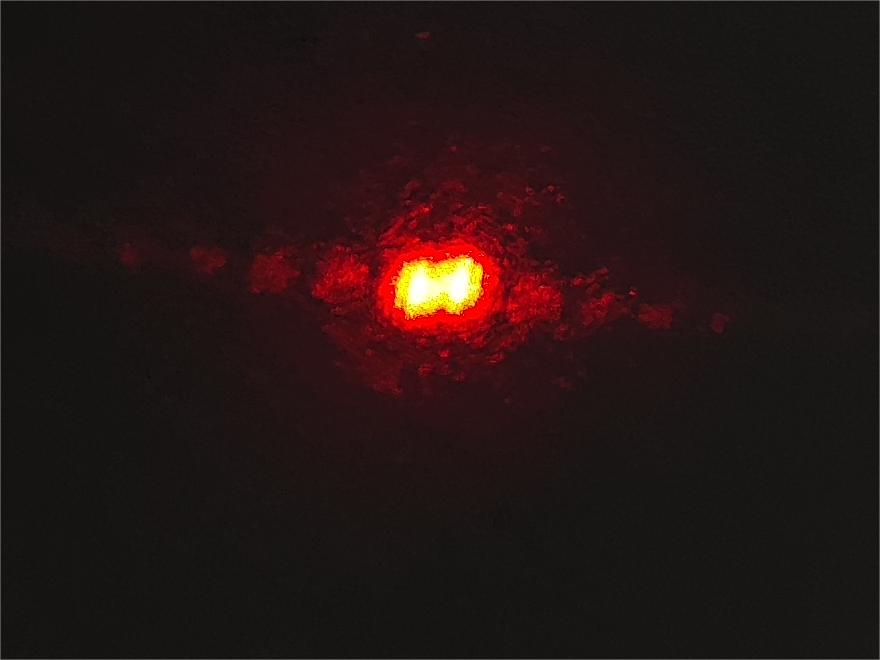
\includegraphics[width=7.5cm]{Fig/3 (22).jpg}}
            \hspace{0.5in}
            \caption{衍射图案}
        \end{figure}
        \begin{figure}[H]
            \centering
            \subfigure[]{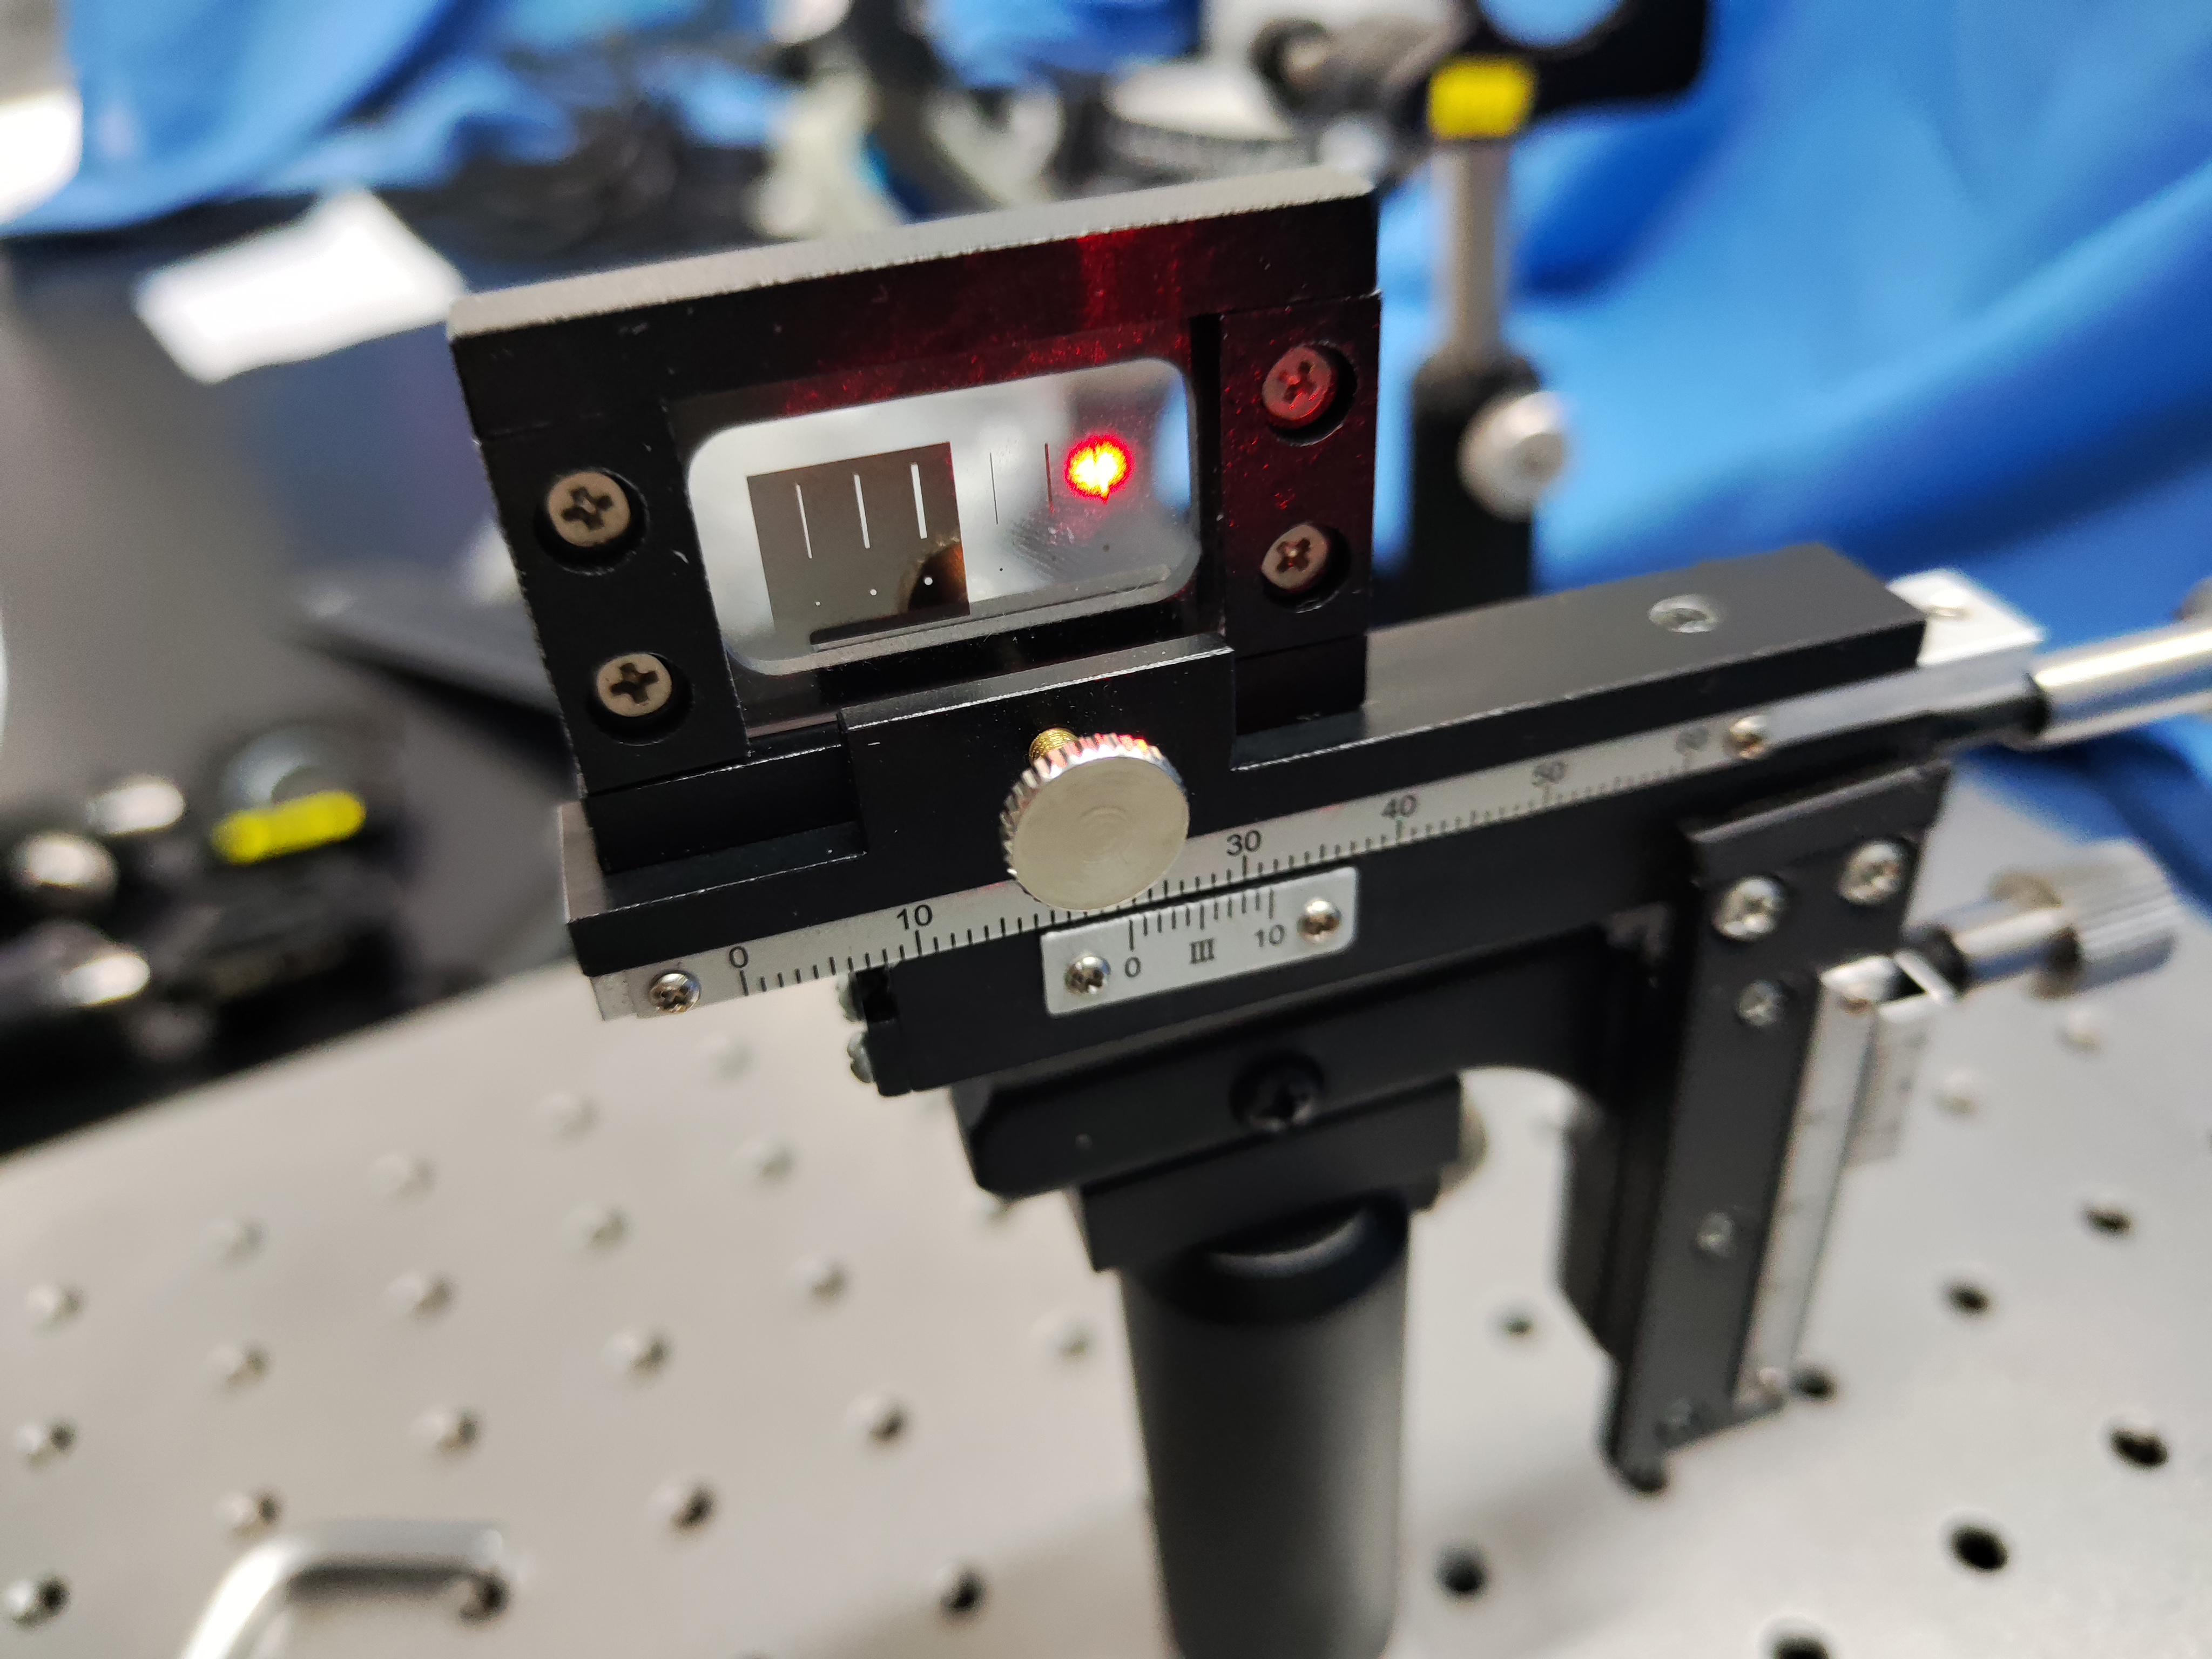
\includegraphics[width=7.5cm]{Fig/3 (23).jpg}}
            \hspace{0.5in}
            \subfigure[]{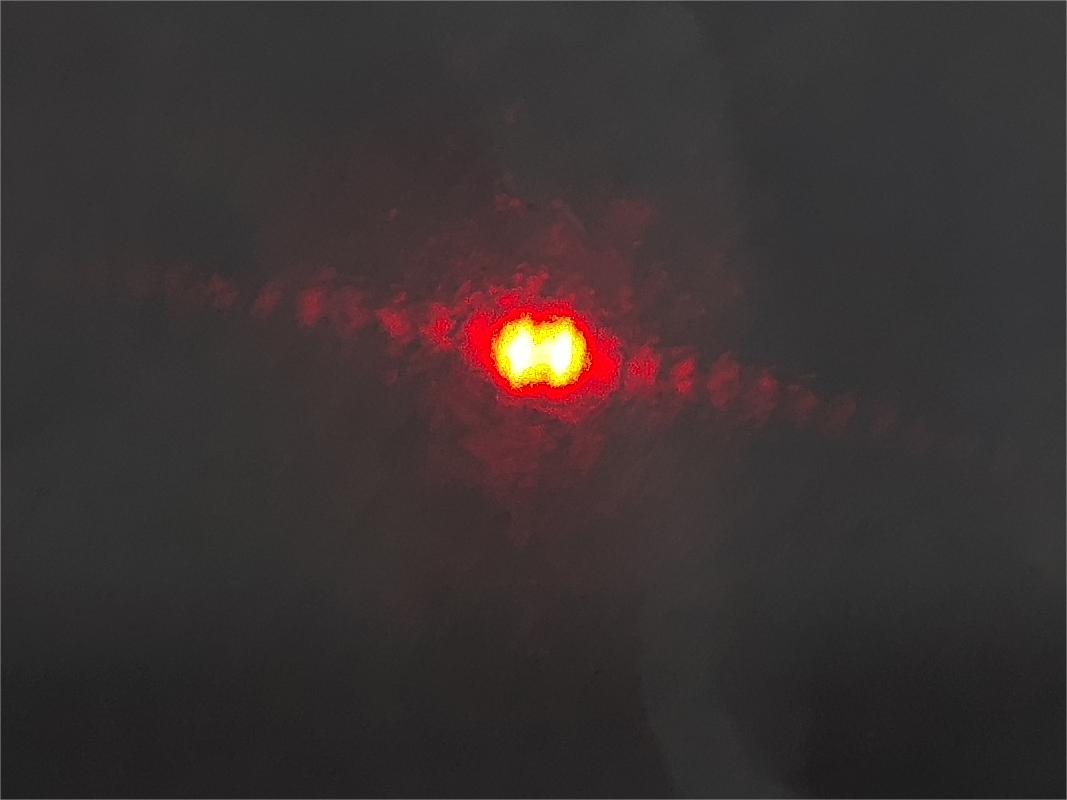
\includegraphics[width=7.5cm]{Fig/3 (24).jpg}}
            \hspace{0.5in}
            \caption{衍射图案}
        \end{figure}
        \begin{figure}[H]
            \centering
            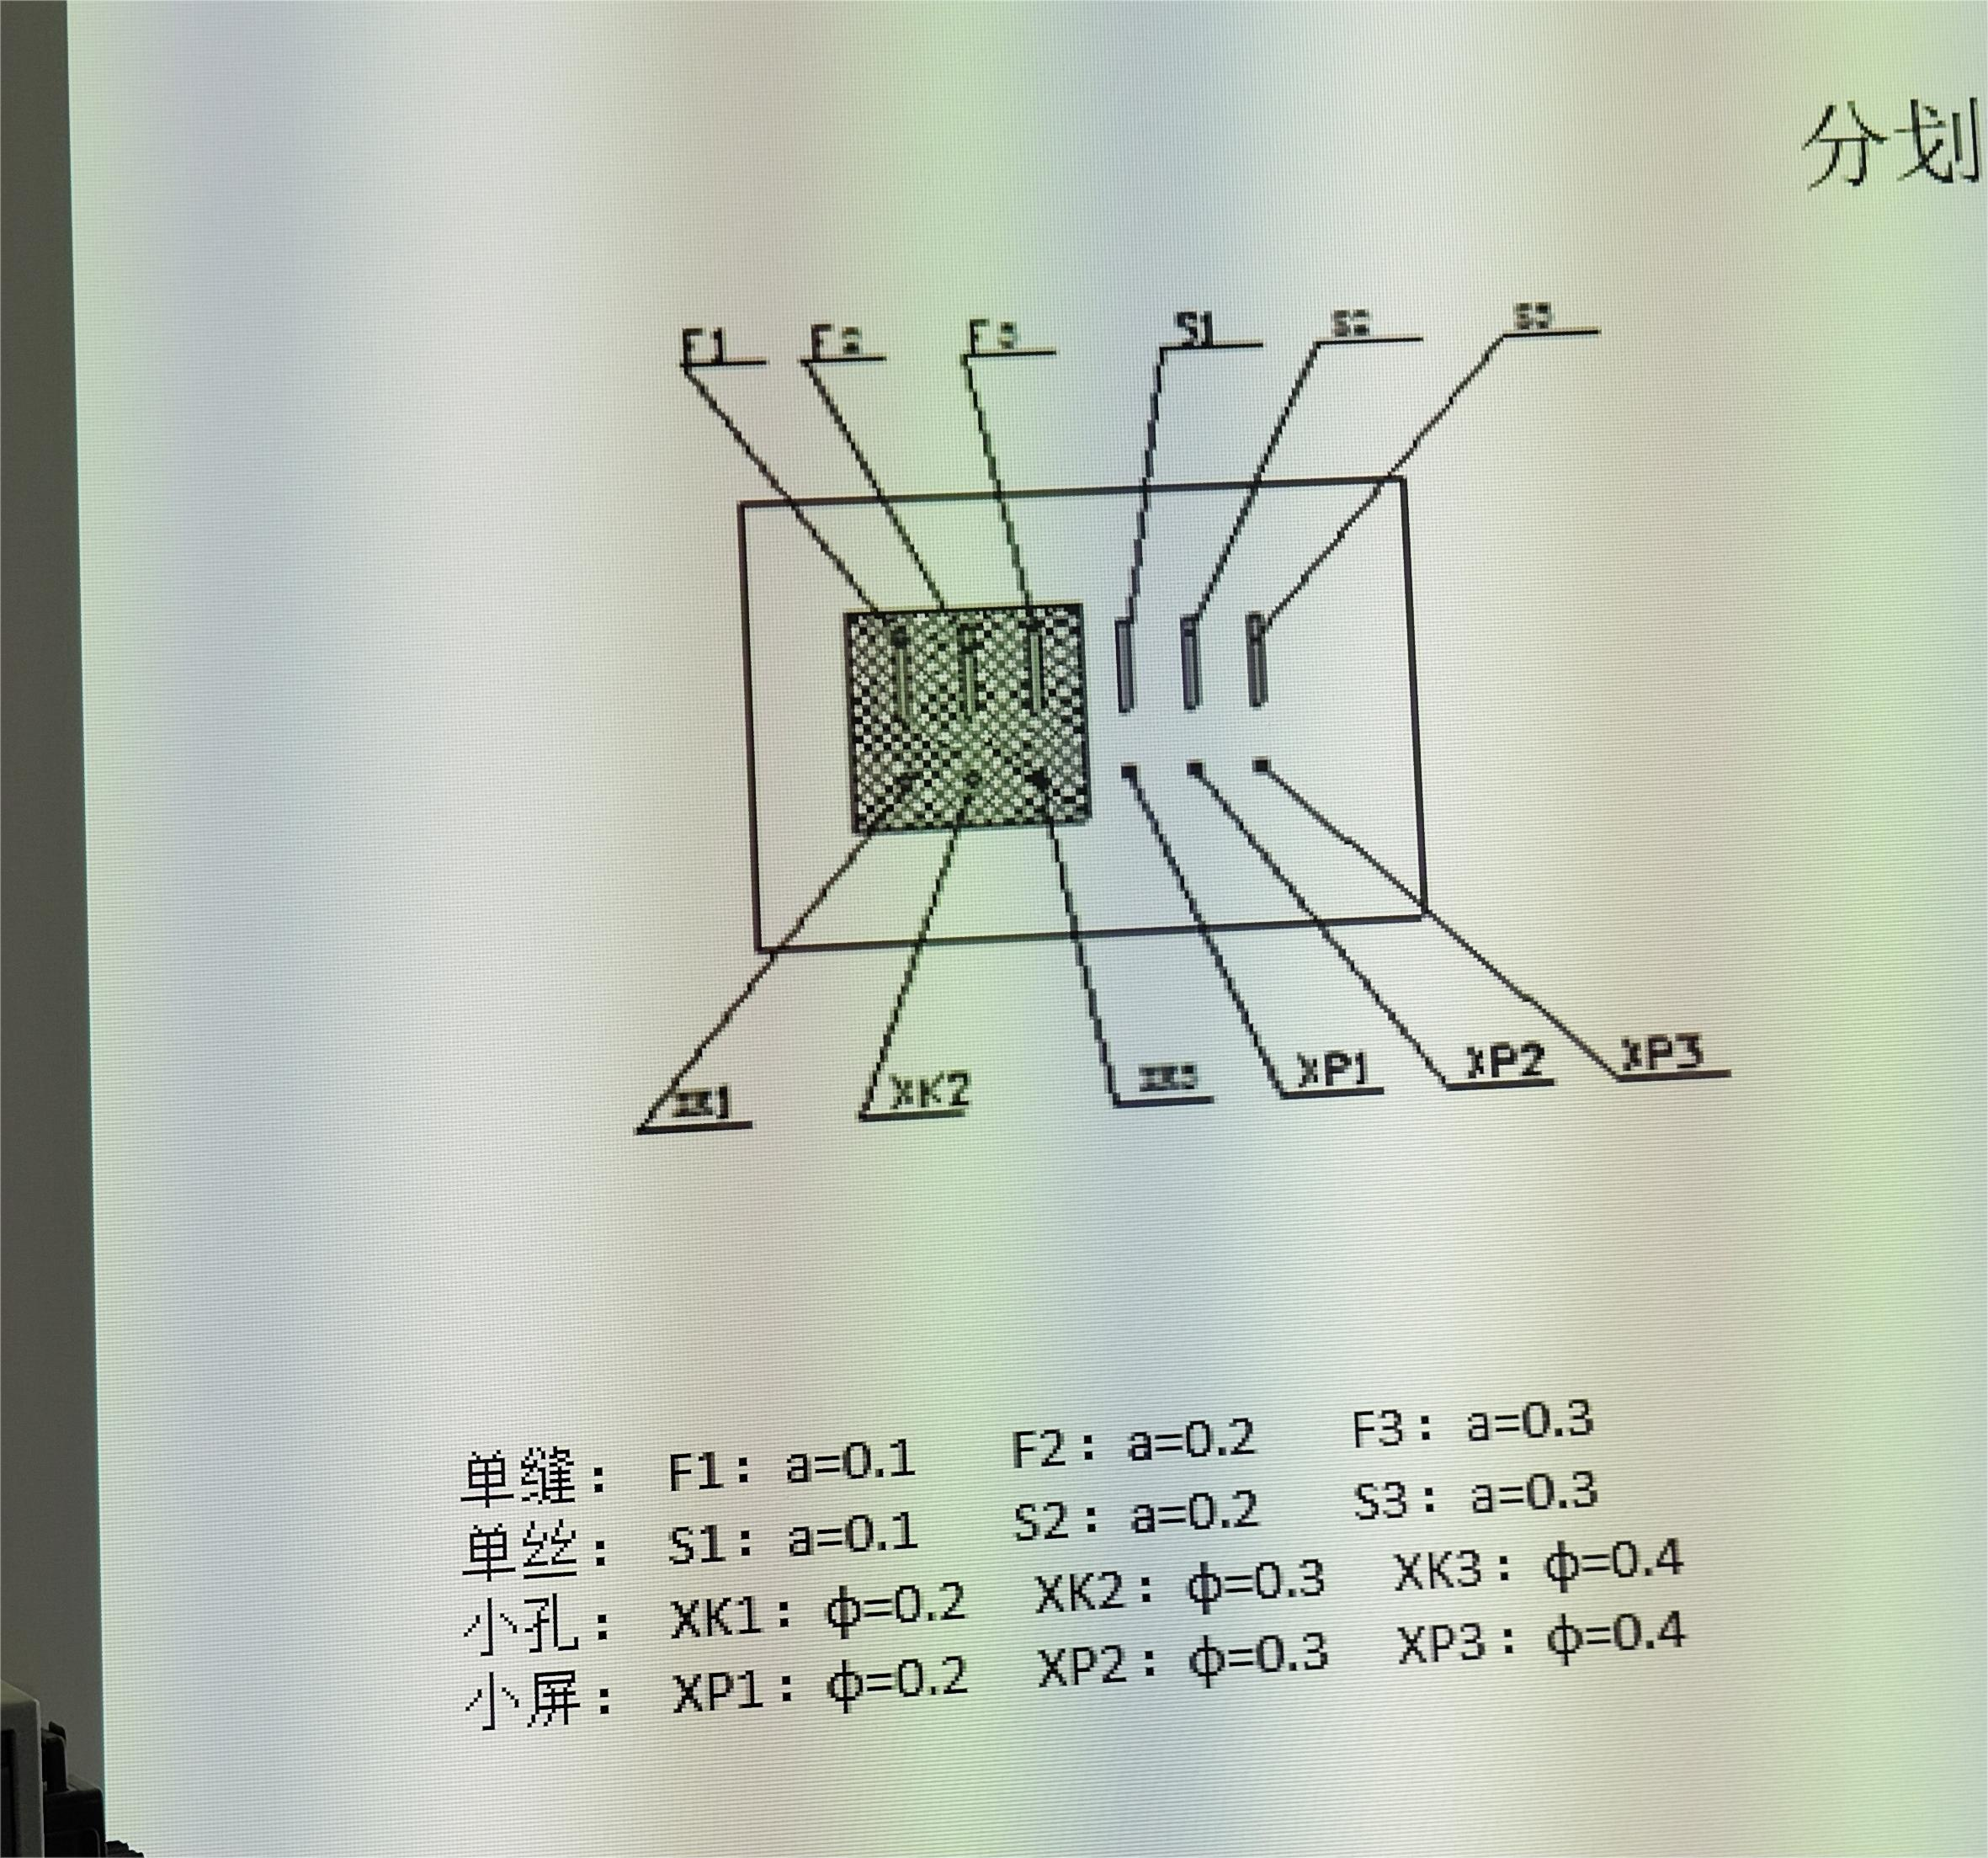
\includegraphics[width=10cm]{Fig/4.jpg}
            \caption{分划板数据}
        \end{figure}
    \end{enumerate}

    \item 光的偏振
    \begin{enumerate}
        \item 移除分划板,将两个偏振片加入光路,调整光路准直后,调整偏振片角度,观察并测量光强变化(角度为偏振片上的刻度,不为实际角度)。理论上,当两个偏振片平行时,光强最大,当两个偏振片垂直时,光强最小。
        \begin{table}[H]
            \centering
            \begin{tabular}{|c|c|c|}\hline
                起偏器角度/(°)&检偏器角度/(°)&$I$/(μA)\\\hline
                0 &0  &3.5 \\\hline
                0 &30  &3.3 \\\hline
                0 &60  &1.8 \\\hline
                0 &90  &410 \\\hline
                0 &120  &430 \\\hline
                0 &150  &1.3  \\\hline
                0 &180  &3.1  \\\hline
                0 &210  &2.8  \\\hline
                0 &240  &1.6  \\\hline
                0 &270  &400   \\\hline
                0 &300  &375   \\\hline
                0  &330  &1.6    \\\hline
               
                
            \end{tabular}
            \caption{光的偏振}
        \end{table}
    \end{enumerate}
\end{enumerate}

\section{实验反思、收获与总结}
\begin{enumerate}
    \item 激光设备有危险性,注意激光落点,不要落到其他组区域,不要试图直视激光。
    \item 调整光路准直需要耐心,要尽量保证光路在同一高度。
\end{enumerate}

\begin{center}
    \vspace*{1em}
    \Large \bf 第二部分\qquad 实验原始记录
\end{center}

\begin{figure}[H]
    \centering
    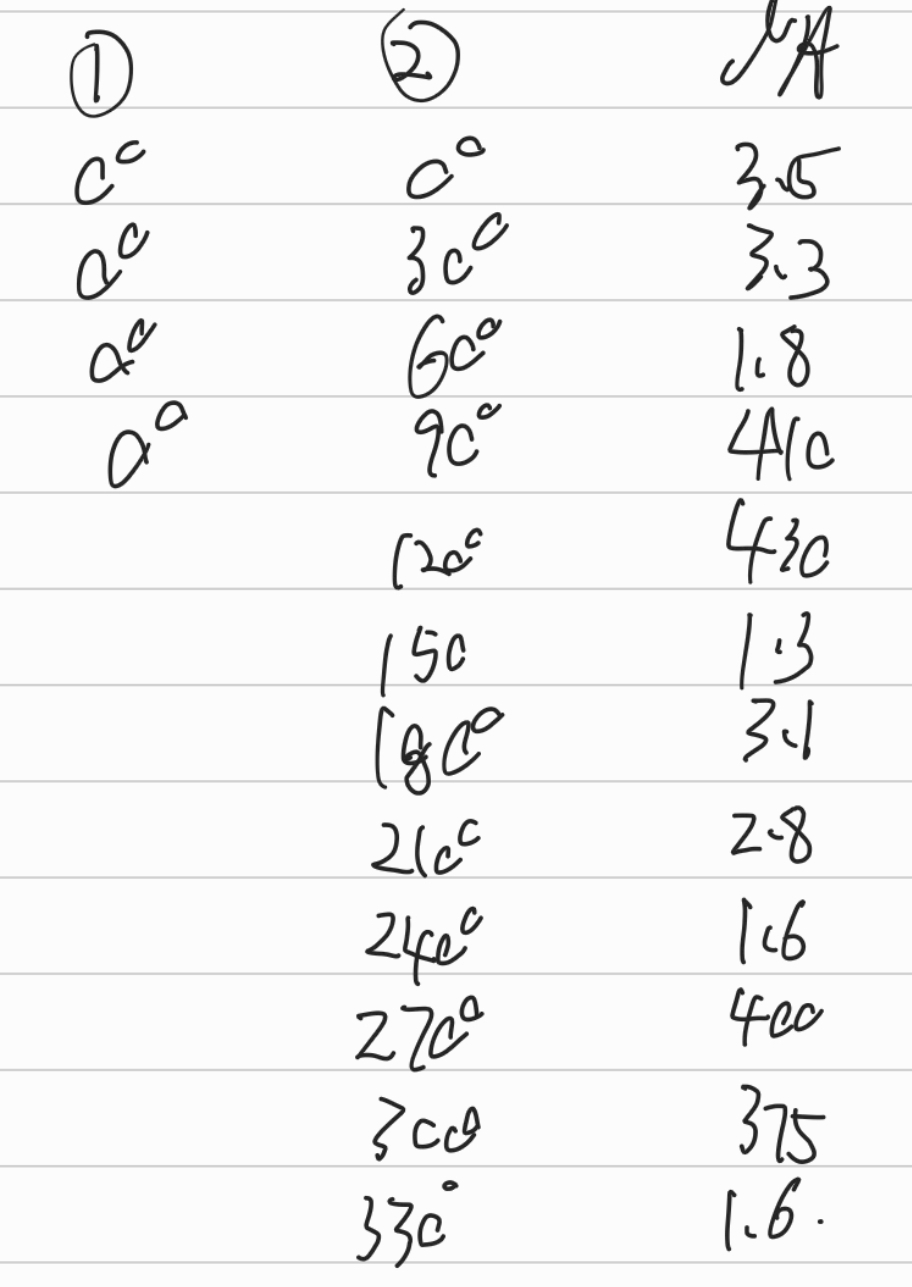
\includegraphics[width=7cm]{Fig/5.jpg}
    \caption{实验记录}
\end{figure}

\end{document}